\documentclass[journal]{IEEEtran}
\usepackage{amsmath,amsfonts}
\usepackage{algorithm}
\usepackage{algorithmic}
\usepackage{array}
\usepackage[caption=false,font=normalsize]{subfig}
\usepackage{textcomp}
\usepackage{stfloats}
\usepackage{url}
\usepackage{verbatim}
\usepackage{graphicx}
\usepackage{cite}
\usepackage{booktabs}
\usepackage{multirow}
\hyphenation{op-tical net-works semi-conduc-tor IEEE-Xplore}

\begin{document}

\title{WiFiLogParser: End-to-End Semantic Parsing of Heterogeneous Wi-Fi Logs for Mobility Data Extraction}

\author{Qingrong Yang,
	Lei Zhu$^{*}$,
	and~Yuqiu Yuan
	\thanks{Q. Yang and Y. Yuan are Ph.D. students with the Department of Industrial and Systems Engineering, The University of North Carolina at Charlotte, Charlotte, NC 28223, USA (e-mail: yqingron@charlotte.edu; yyuan7@charlotte.edu).}
	\thanks{$^{*}$Lei Zhu is the corresponding author and is an Assistant Professor with the Department of Industrial and Systems Engineering, The University of North Carolina at Charlotte, Charlotte, NC 28223, USA (e-mail: Lei.Zhu@charlotte.edu).}}

\markboth{IEEE Access,~Vol.~XX, No.~X, XXXX~2026}%
{Yang \MakeLowercase{\textit{et al.}}: WiFiLogParser}

\maketitle

\begin{abstract}
	In public Wi-Fi deployments, logs record Wi-Fi client and access point (AP) interactions at scale and therefore encode mobility signals for hotspot and flow analytics. However, extracting the embedded human mobility patterns from heterogeneous Wi-Fi logs is challenging. Log parsing turns free-form system logs into structured records for downstream analysis. Yet most general-purpose log parsers stop at template extraction, leaving unresolved issues, like communicating event typing and role-aware field semantics, which are needed to convert Wi-Fi logs into mobility records. WiFiLogParser, a large language model (LLM)-based framework, is proposed to extract the key information, such as timestamps and AP and client identifiers (name, IP, and MAC), directly from raw Wi-Fi logs without prior format specifications. WiFiLogParser couples iterative timestamp-header induction with structural signature micro-grouping and greedy consolidation to learn reusable parsers and applies a bounded self-repair loop when patterns fail validation. Across three real-world datasets from different Wi-Fi vendors, WiFiLogParser achieves F1-scores of 0.916–0.999 and field extraction accuracy (FEA) of 0.924–1.000 on complete datasets.  Relative to a Direct LLM baseline, WiFiLogParser reduces token consumption by over 99\% and cuts API calls and LLM-only runtime by more than 98\% in per-1,000-line cost estimates.
\end{abstract}

\begin{IEEEkeywords}
	Wi-Fi logs, log semantic parsing, large language model, regular expressions, human mobility data.
\end{IEEEkeywords}

\section{Introduction}
\IEEEPARstart{P}{ublic} Wi-Fi services are widely deployed in airports, campuses, hospitals, and city centers, and they sit at the operational core of many smart-city and Internet of Things (IoT) infrastructures \cite{ref1,ref2,ref3}. The logs these systems generate are usually read as artifacts for network operations and troubleshooting, yet they also record rich client--AP interactions (e.g., join/leave, authentication/association, and disassociation/deauthentication) \cite{zhu2025exploring, ref6}. Seen through a mobility lens, those interactions supply temporal (\emph{when}) and spatial (\emph{where}) signals that can be transformed into mobility records for downstream analytics, such as flow estimation and hotspot analysis \cite{ref4,ref5,ref9}.

Converting Wi-Fi logs into structured mobility records involves more than straightforward string matching. The process must operate at scale, accommodate heterogeneous log formats, and preserve mobility-relevant semantics. In large Wi-Fi systems, gigabytes of logs can be generated within hours, making manual rule-based parsing infeasible. At the same time, Wi-Fi vendors expose logs in diverse formats, including free-text syslog messages, key–value pairs, CSV-like exports, and embedded JSON. Documentation of these formats is often incomplete or unavailable \cite{ref14,ref15}, which complicates the design of stable extraction rules. Beyond structural variability, mobility extraction further requires accurate event typing and role-specific field identification (e.g., distinguishing AP and client identifiers).

In recent years, large language models (LLMs) have made significant progress in the field of log parsing due to their powerful semantic understanding capabilities. They parse log samples and represent all samples with a template library, which helps in parsing Wi-Fi logs to extract mobility records. However, token-based pricing made early line-by-line parsing prohibitively expensive \cite{ref43}. By grouping logs, LILAC \cite{ref30} and LogBatcher \cite{ref32} can parse the entire log dataset at lower cost. However, these existing parsers still have three limitations for Wi-Fi mobility extraction.



(1) Existing parsers focus on inducing templates by separating constants from variables \cite{ref22}. However, in Wi-Fi mobility extraction, the parser must identify the event type and role-specific fields for APs and clients. Traditional parsers do not provide these role-specific fields and often treat the event token as a variable \cite{ref30,ref32}, thereby losing event semantics. This makes the events hard to identify at the template level, which limits their use for Wi-Fi mobility extraction. Fig.~\ref{fig:brain_mix} shows a common failure mode: distinct Wi-Fi event types are grouped together because they share a similar structure, resulting in more difficult event identification and role-specific field extraction.

\begin{figure}[!t]
	\centering
	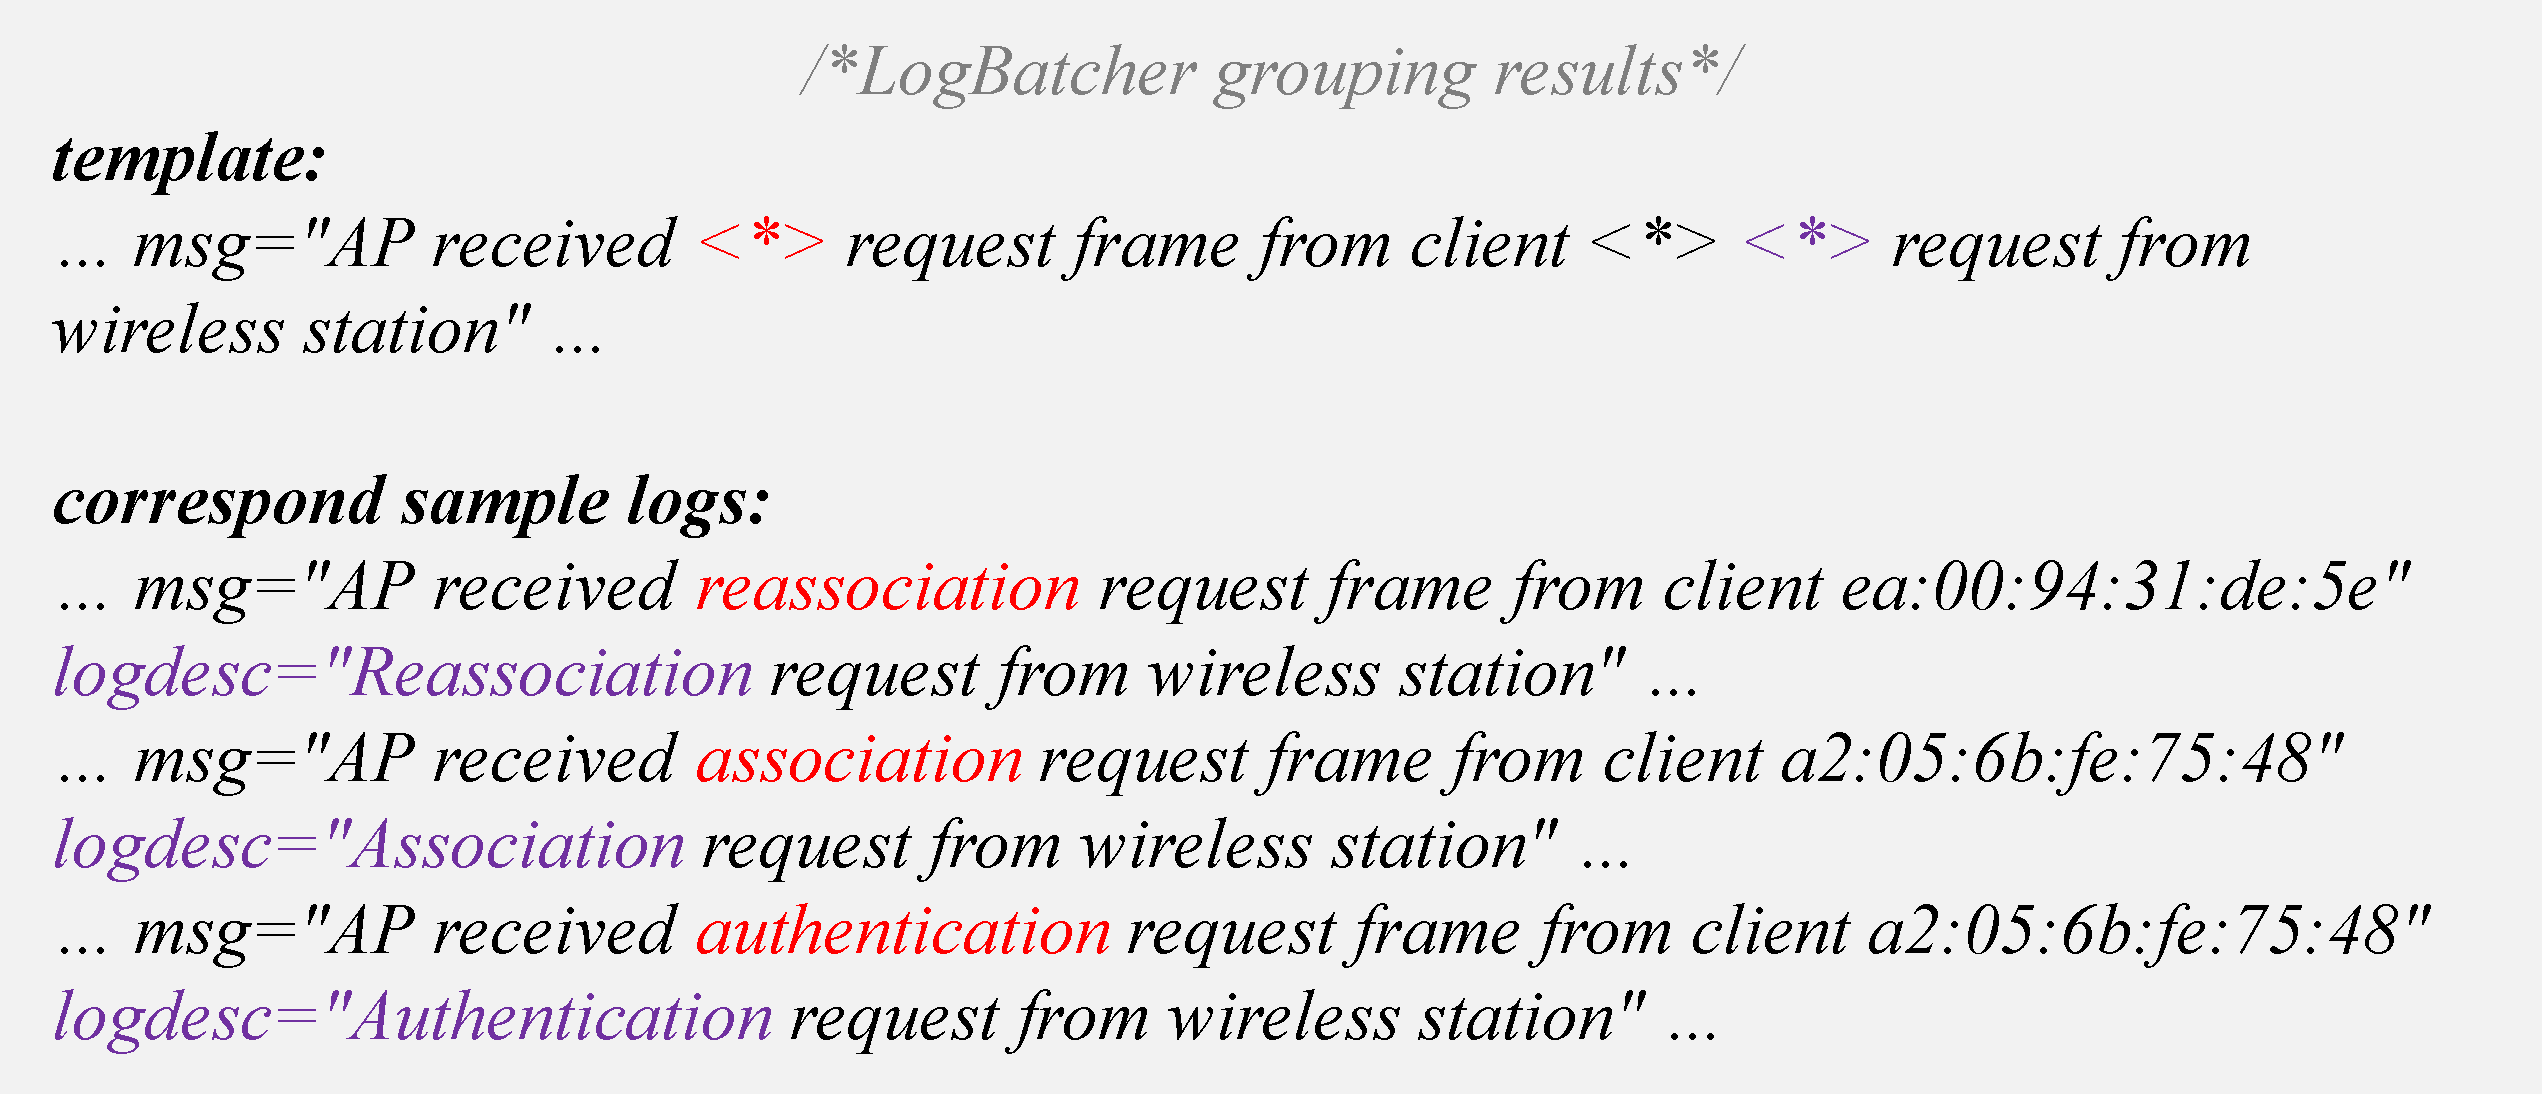
\includegraphics[width=\linewidth]{figure/Picture2.pdf}
	\caption{Example: different Wi-Fi event types are grouped together by token frequency (example from LogBatcher \cite{ref32}).}
	\label{fig:brain_mix}
\end{figure}

(2) Existing parsers typically group logs based on token similarity or edit distance, which fails to ensure semantic purity \cite{ref18,ref23,ref47,ref22}. In Wi-Fi logs, semantically different events may exhibit highly similar token similarity or edit distance, leading to event-grouping confusion, and these errors subsequently propagate to all lines within the group.

(3) Existing parsers typically treat headers containing timestamps as known parameters \cite{ref22,ref44}. However, the real-world logs usually do not provide explicit timestamp format specifications. A common practice is to manually write extraction rules, which is slow and hard to maintain. Timestamps are important for Wi-Fi mobility analysis, enabling sorting, session reconstruction, and mobility inference. Therefore, developing a stable timestamp extraction method is necessary.


To address these issues, we developed WiFiLogParser, an end-to-end framework that directly extracts mobility records from raw logs. WiFiLogParser first induces a timestamp header pattern using LLM and removes header metadata. It then groups logs into high-purity micro-groups using a structural signature. For each micro-group, it uses LLM to induce a reusable parser that includes a regular expression (regex) and an event label. Finally, it consolidates fragmented micro-groups using regex-coverage validation, including those that have not been parsed yet, to save time and reduce cost. Fig.~\ref{fig:compare} contrasts traditional log parsing with our method.


\begin{figure}[!t]
	\centering
	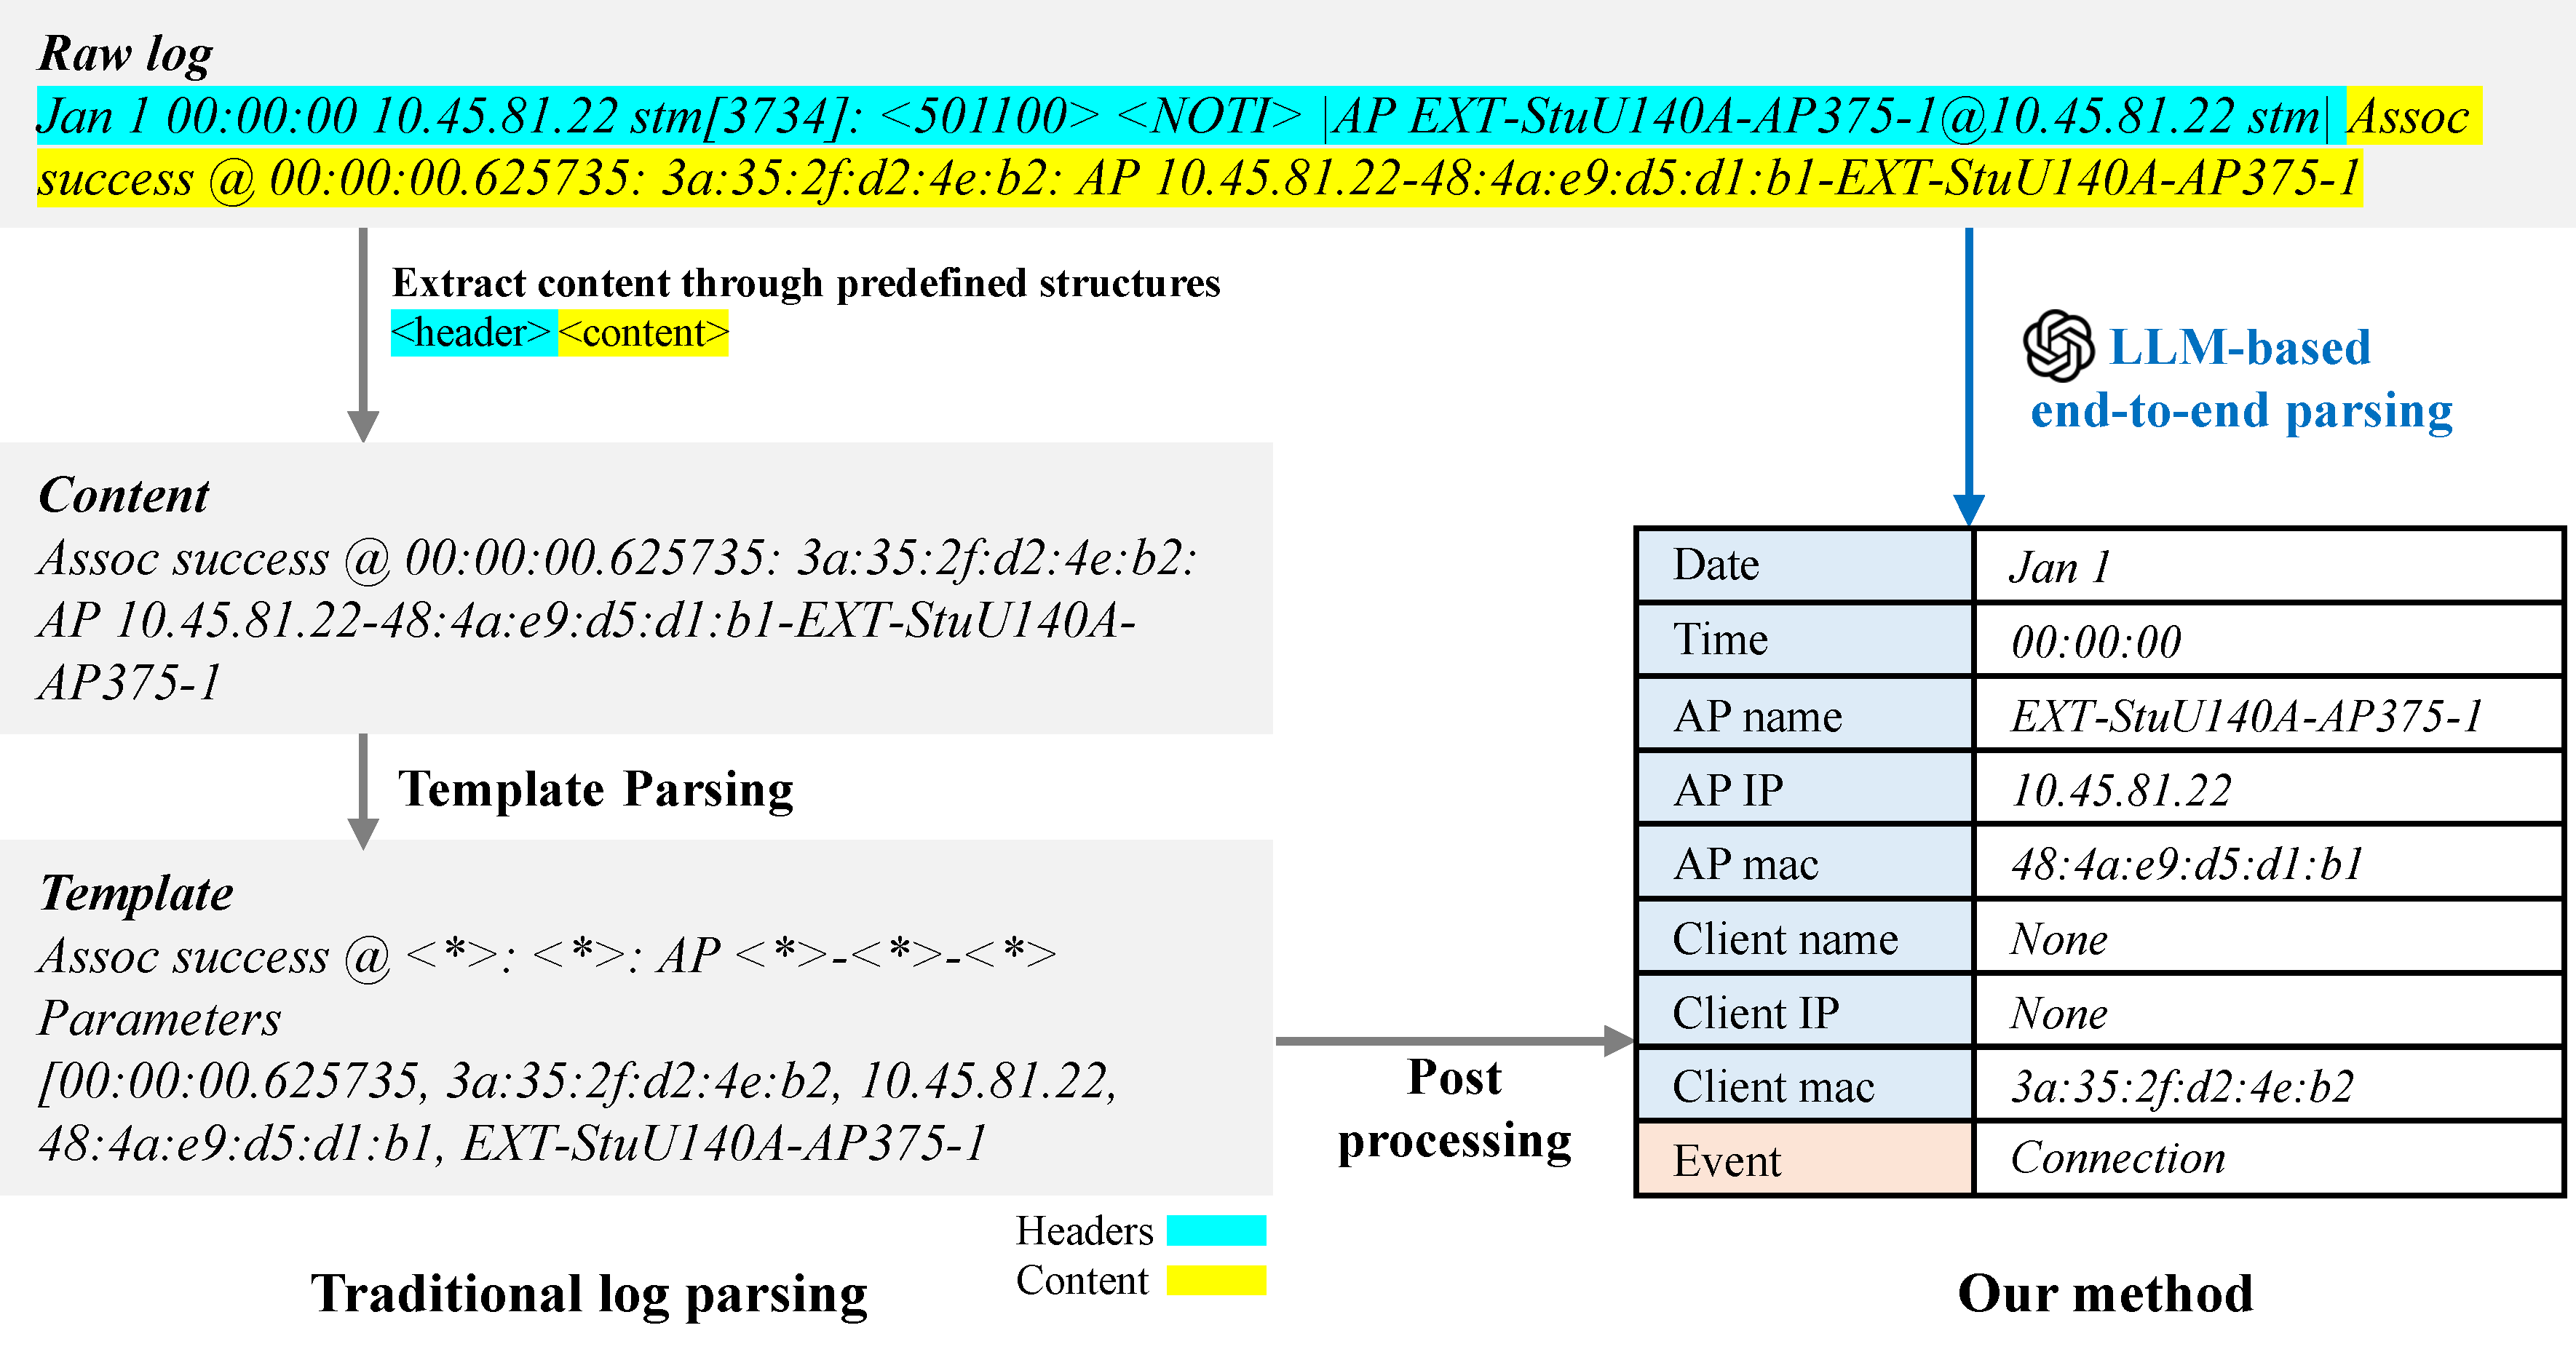
\includegraphics[width=\linewidth]{figure/Picture1.pdf}
	\caption{Comparison between WiFiLogParser and traditional parsing methods.}
	\label{fig:compare}
\end{figure}


We make three contributions:
\begin{itemize}
	\item \textbf{Automatic timestamp header induction.} We propose an LLM-driven, coverage-guided procedure to induce a timestamp header regex without vendor-specific format manuals, enabling robust header/content separation.
	\item \textbf{Split-for-purity parsing with greedy consolidation.} We design a scalable pipeline that induces parsers (named-group regex and event labels) from high-purity structural micro-groups, then greedily consolidates fragmented groups using regex coverage validation and caching.
	\item \textbf{Empirical evaluation on real deployments.} We evaluate WiFiLogParser on three real-world Wi-Fi log datasets from different vendors, reporting event F1, field extraction accuracy, and efficiency/cost statistics at both small and million-scale settings.
\end{itemize}

\section{Related Work}
\subsection{Traditional Log Parsing}
Traditional log parsing largely treats the problem as template discovery: raw messages are abstracted into invariant patterns via token heuristics, tree structures, and clustering. Most systems follow a clustering-first workflow, grouping messages by syntactic similarity and then deriving templates within each cluster. Representative methods include Drain \cite{ref17}, IPLoM \cite{ref47}, LenMa \cite{ref48}, LogMine \cite{ref23}, Logram \cite{ref21}, and Brain \cite{ref16}. Drain uses fixed-depth parsing trees for efficient online matching; IPLoM performs iterative partitioning based on token positions; Logram builds $n$-gram dictionaries to improve robustness. Beyond clustering-first designs, pattern/signature mining methods such as LogCluster \cite{ref20} and LogSig \cite{ref49} mine frequent patterns directly from raw logs. For streaming and incremental parsing, Spell \cite{ref18} and SHISO \cite{ref50} update templates as logs arrive, while MoLFI \cite{ref51} frames log format identification as a search/optimization problem.

These parsers are scalable and mature, but their output is a generic template inventory and does not directly yield the event semantics and role-aware AP/client fields required for Wi-Fi mobility extraction. For that reason, we do not treat them as end-to-end baselines: mapping templates to our schema would require additional domain heuristics and would introduce extra variance. This choice is also consistent with benchmarking and evaluation guidelines showing that reported conclusions can be sensitive to preprocessing and evaluation protocols \cite{ref22,ref45,ref46}.

\subsection{LLM-based Log Parsing}
Large language models bring semantic reasoning to log text and have recently been adopted for template induction. Prompt-based parsing and comparative studies suggest that LLMs can reduce reliance on handcrafted rules \cite{ref31,ref33,ref54,ref52}. Several systems go beyond direct prompting: LogParser-LLM studies efficient log parsing with LLMs \cite{ref26}, and Lemur explores LLM-assisted template merging \cite{ref34}. Cost remains a first-order constraint. Na\"ive per-line prompting scales poorly with log volume, which motivates batching and caching strategies such as demonstration-free prompting \cite{ref37}, LogBatcher-style batch parsing \cite{ref32}, and LILAC's adaptive parsing cache \cite{ref30}. Other lines of work study unsupervised LLM parsers and open-source deployments \cite{ref53,ref35}.

A recent review surveys 29 LLM-based log parsing methods, benchmarks seven of them, and reports that LogBatcher achieves the best performance across metrics, followed by LILAC among the compared methods \cite{ref44}.

Notwithstanding their strengths, these systems primarily optimize template extraction. For Wi-Fi mobility analytics, templates must still be translated into event types and role-aware field mappings. WiFiLogParser targets this end task directly by inducing executable regex with named groups and validating them at the micro-group level.

\subsection{Wi-Fi Logs for Mobility}
Wi-Fi sensing and network records have been used as a cost-effective source of human mobility signals for flow estimation, hotspot analysis, and public health monitoring \cite{ref1,ref4,ref9,ref3}. Much of this literature assumes that mobility records (timestamp, device identifier, and location/AP identifier) are already available or can be obtained from structured Wi-Fi records (e.g., probe-based traces). Operational deployments complicate that assumption: the raw data is often exposed as heterogeneous system logs whose formats vary across vendors and configurations. WiFiLogParser addresses this gap by extracting mobility records directly from raw Wi-Fi logs with minimal format assumptions.

\section{Problem Formulation}
We consider a collection of raw Wi-Fi log lines $L = \{l_1, l_2, \ldots, l_n\}$ with unknown vendor-specific formats. The goal is to produce a structured mobility record for each line:
\begin{equation}
	\mathrm{parse}(l_i) \rightarrow (y_i, \mathbf{v}_i),
\end{equation}
where $y_i \in \{1, -1, 0\}$ is an event label (1: connection-related, -1: disconnection-related, 0: other), and $\mathbf{v}_i$ contains seven extracted fields:
{timestamp, ap\_name, ap\_ip, ap\_mac, client\_name, client\_ip, client\_mac}.
If a field is not present in a log line, the correct output for that field is an empty value.

Wi-Fi logs may include identifiers in different forms (names, IPs, and MACs) and may mention multiple devices in the same message (e.g., the logging source, the AP involved in the event, and the client device). Our task isolates the event participants: AP and client involved in the connectivity event. Because vendor naming conventions and surface tokens differ, a practical parser must infer whether the role is AP or client and field types (name/IP/MAC) from context rather than relying on fixed keywords.

\section{Method}
\subsection{Framework Overview}

For clarity, we use the following terminology consistently throughout this paper. A structural signature (also called a skeleton) denotes the masked content string obtained after applying the masking rules in Table~\ref{tab:skeleton_rules}. Logs sharing the same structural signature form one micro-group. A parser denotes a pair of an executable full-line regular expression and an event label. A parser bucket denotes one or more micro-groups that share the same validated parser after consolidation. We use the term template only when referring to prior template-oriented parsers.

Fig.~\ref{fig:overview} summarizes WiFiLogParser as a four-step pipeline. The guiding choice is to use the LLM to induce reusable parsers (regex and event label) rather than parsing each line independently. Once learned, the regex can be applied deterministically across many lines.

\begin{figure*}[!t]
	\centering
	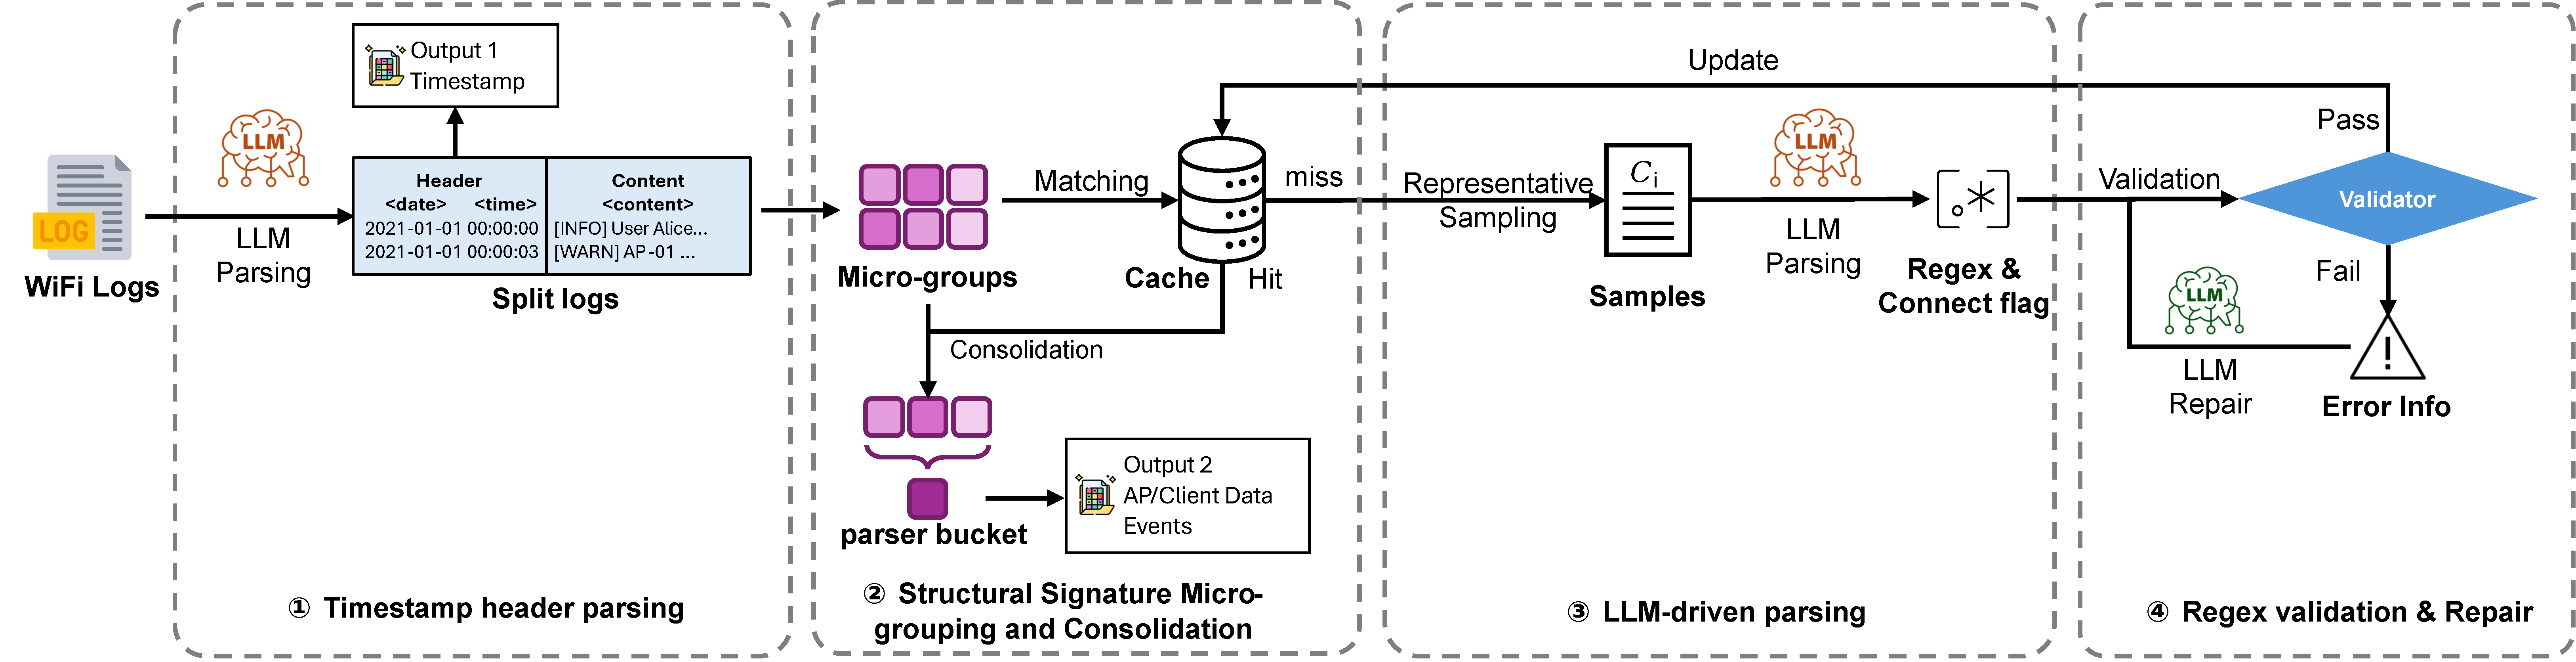
\includegraphics[width=\textwidth]{figure/pipeline.pdf}
	\caption{WiFiLogParser pipeline overview. Step 1 splits each raw log into timestamp header/content and outputs the timestamp. Step 2 forms micro-groups through structural signature and uses cache matching with consolidation to build parser buckets and extract AP/client fields and events when possible. Step 3 induces a parser (regex + event label) from representative samples for cache misses. Step 4 validates and self-repairs regex; validated parsers update the cache for reuse.}
	\label{fig:overview}
\end{figure*}

\subsection{Step 1: Timestamp Header Parsing}
WiFiLogParser begins by separating each raw line into a timestamped header and a semantic content message. Because header formats vary across vendors, we prompt the LLM to infer an anchored regex $H$ that matches the full line and exposes named groups for "date", "time", and "content". Step~1 in Fig.~\ref{fig:overview} illustrates this process. For sampled lines, the LLM proposes an anchored header regex that extracts date, time, and content. We then combine date and time and parse the timestamp using the dateutil parser \cite{ref56} via pandas.to\_datetime \cite{ref57}. We then forward only the content to subsequent steps.

We perform diversity sampling using determinantal point processes (DPP) \cite{ref36}, where the similarity kernel is constructed from TF-IDF representations with cosine similarity, following the formulation in LogBatcher \cite{ref32}. From this diverse subset, we prompt the LLM to propose an anchored header regular expression. If the resulting header $H$ does not cover all lines, we iteratively refine $H$ using uncovered lines until achieving high coverage ($\tau = 95\%$). Appendix~A provides a pseudocode sketch.

\subsection{Step 2: Structural Signature Micro-grouping and Consolidation}

\textbf{Structural Signature Micro-grouping}:
After stripping the timestamp header (Step~1), WiFiLogParser groups lines using a structural signature designed to produce high-purity micro-groups. Concretely, we apply a sequence of variable-masking rules to remove common high-variance tokens, as shown in Table~\ref{tab:skeleton_rules}. The remaining masked string is treated as a skeleton, and logs with identical skeletons fall into the same micro-group.

\begin{table}[!t]
	\centering
	\caption{Structural signature masking categories (applied sequentially) and examples.}
	\label{tab:skeleton_rules}
	\begin{tabular}{@{}ll@{}}
		\toprule
		\textbf{Category} & \textbf{Example}  \\
		\midrule
		IP                & 192.168.1.1       \\
		MAC               & aa:bb:cc:dd:ee:ff \\
		Website           & example.com       \\
		Hex               & 0x1a2b3c          \\
		Digits            & 123               \\
		Paths             & /log/system.log   \\
		Names$^*$         & Win12-AP34-5      \\
		\bottomrule
	\end{tabular}
	\\[0.2em]
	\footnotesize{$^*$Hyphen/underscore-separated strings often encode device/network names.}
\end{table}

The payoff of structural signatures is intra-group consistency, which stabilizes parser induction and regex validation. To keep the system scalable, WiFiLogParser processes logs in fixed-size chunks (50,000 lines per chunk in our implementation, following practical batching choices in prior work \cite{ref32}) and maintains a persistent parser cache so that validated parsers are reused across chunks. For each micro-group, we first look up a parser by structural signature; on a cache hit, the cached parser deterministically yields the event label and AP/client fields.

In Wi-Fi logs, structural signature grouping can fragment when entity values (e.g., SSIDs and AP names) or embedded payloads (e.g., inline JSON fragments) shift surface patterns. WiFiLogParser compensates with coverage-driven consolidation, merging multiple micro-groups into a shared parser bucket when they are covered by the same validated parser.

\textbf{Coverage-driven Consolidation}:
To address structural signature fragmentation, we use a three-step consolidation procedure for each validated parser \(p\). First, for every unmatched micro-group \(g'\), we test \(p\) on the first line and keep only micro-groups that pass. Second, we apply the parser \(p\) to all lines in each surviving \(g'\); only micro-groups with complete coverage are accepted. Third, we merge each accepted \(g'\) into the parser bucket of \(p\), so these micro-groups share one cached parser. This split-then-merge design preserves purity during micro-group formation while recovering completeness by reunifying semantically identical but surface-fragmented groups.

\subsection{Step 3: LLM-driven Parsing}
WiFiLogParser calls the LLM at the micro-group level. To avoid overfitting to a single instance, we apply the same DPP-based diversity sampling strategy as in timestamp induction to select representative samples for LLM parsing.

For each cache-miss micro-group, WiFiLogParser prompts the LLM to output a parser consisting of (i) an executable full-line regex and (ii) a connectivity flag (event label) $y\in\{1,-1,0\}$. The regex is learned on the \emph{content string} (after timestamp header stripping) and introduces named capture groups for the six fields (AP/client name, IP, and MAC), while the timestamp is taken from Step~1. We constrain the regex representation to favor stability and reuse: (i) the regex must match the full line from beginning to end, (ii) only non-greedy wildcards are used for variable spans, and (iii) named capture groups are only permitted for the target schema fields.

\subsection{Step 4: Regex Validation and Self-Repair}
WiFiLogParser validates the generated regex against all lines in the originating micro-group. If any line fails to match, we localize the mismatch and provide a compact diagnostic to the same LLM for self-repair under a retry budget. In our implementation, we localize failures by incrementally matching delimiter-bounded regex segments to estimate a mismatch position and return a short context window. Upon successful validation, the parser is added to the cache (structural signature index and parser library) for reuse. The self-repair loop is bounded to avoid excessive retries; groups that still fail after the budget are flagged for audit. Appendix~B provides a pseudocode sketch. The prompt structure sketches used in timestamp induction, parser induction, and self-repair are shown in Fig.~\ref{fig:prompt_sketch}.


\begin{figure}[!t]
	\centering
	\subfloat[Timestamp header induction prompt structure]{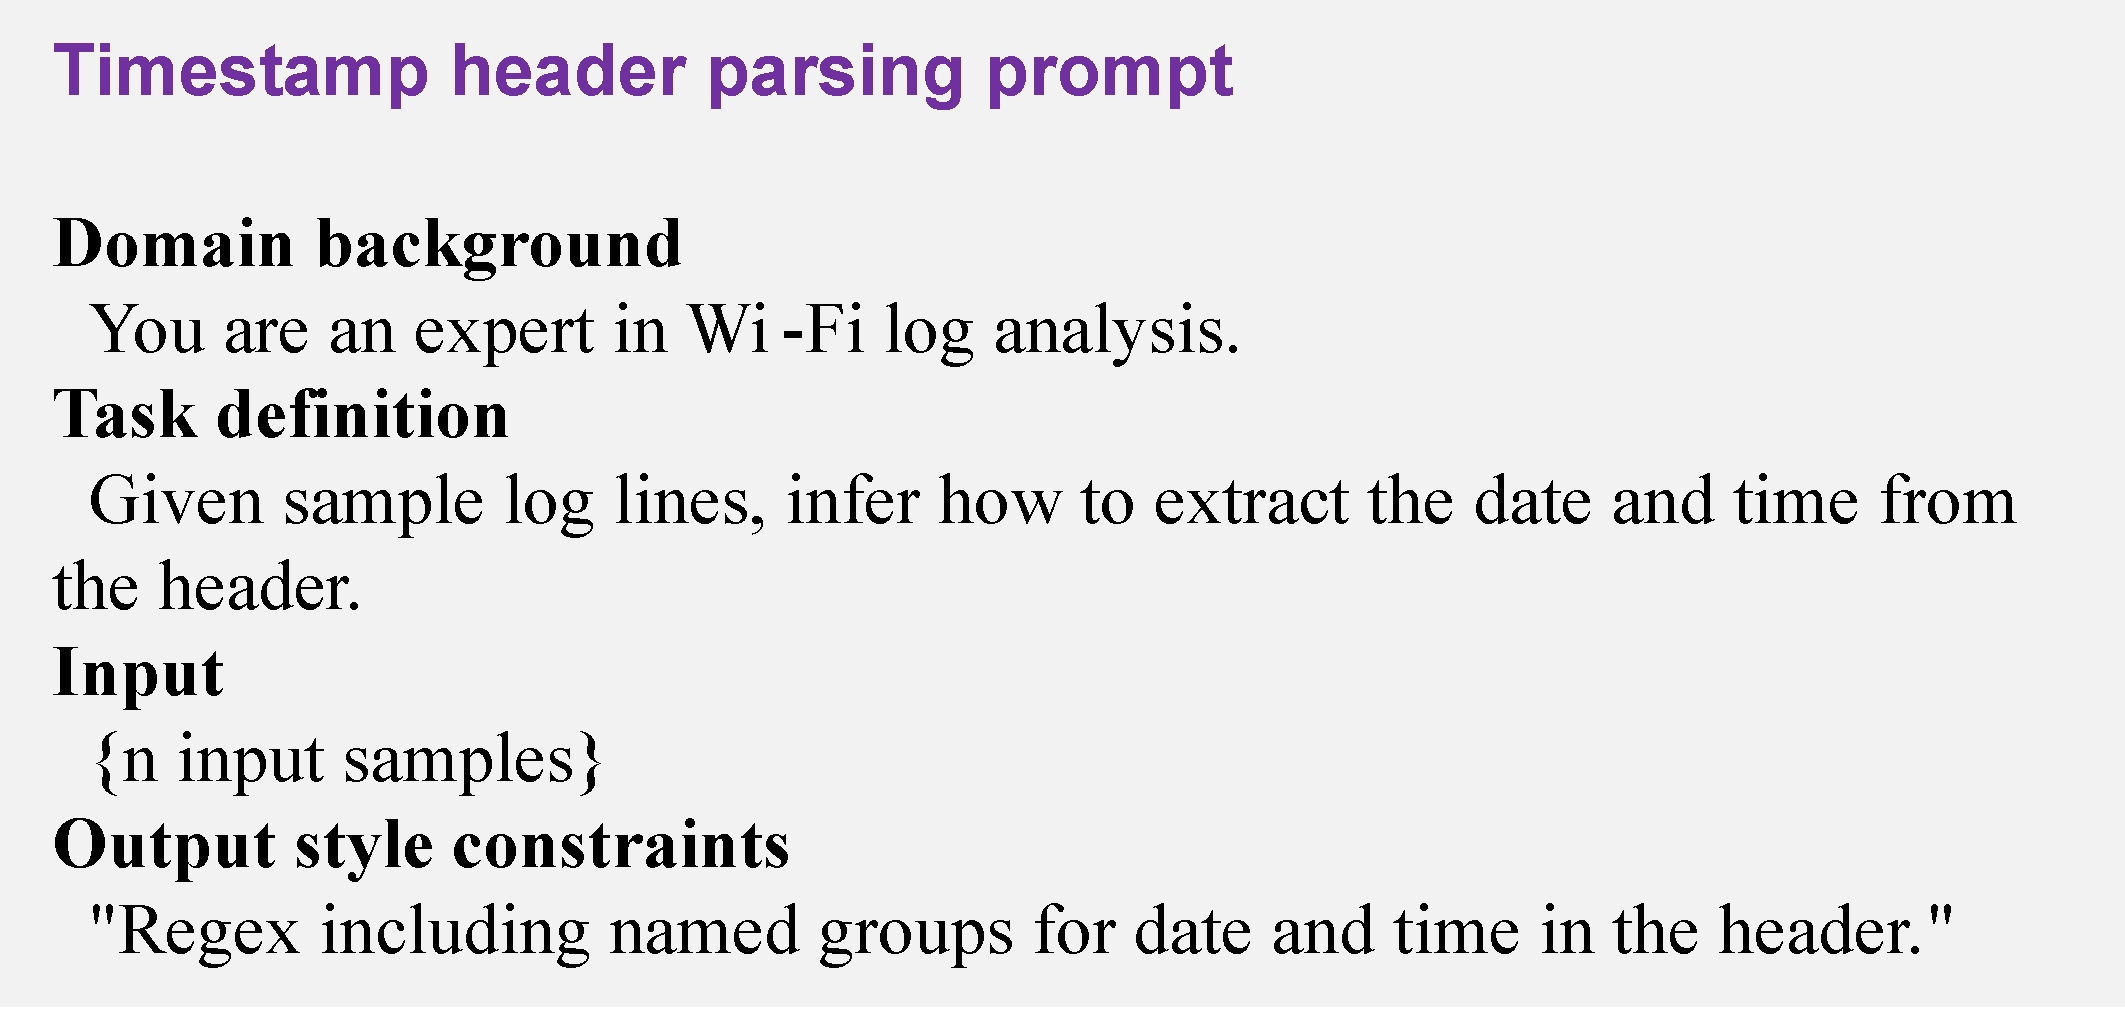
\includegraphics[width=0.95\linewidth]{figure/Picture5.pdf}}\\[0.6ex]
	\subfloat[LLM parsing prompt structure]{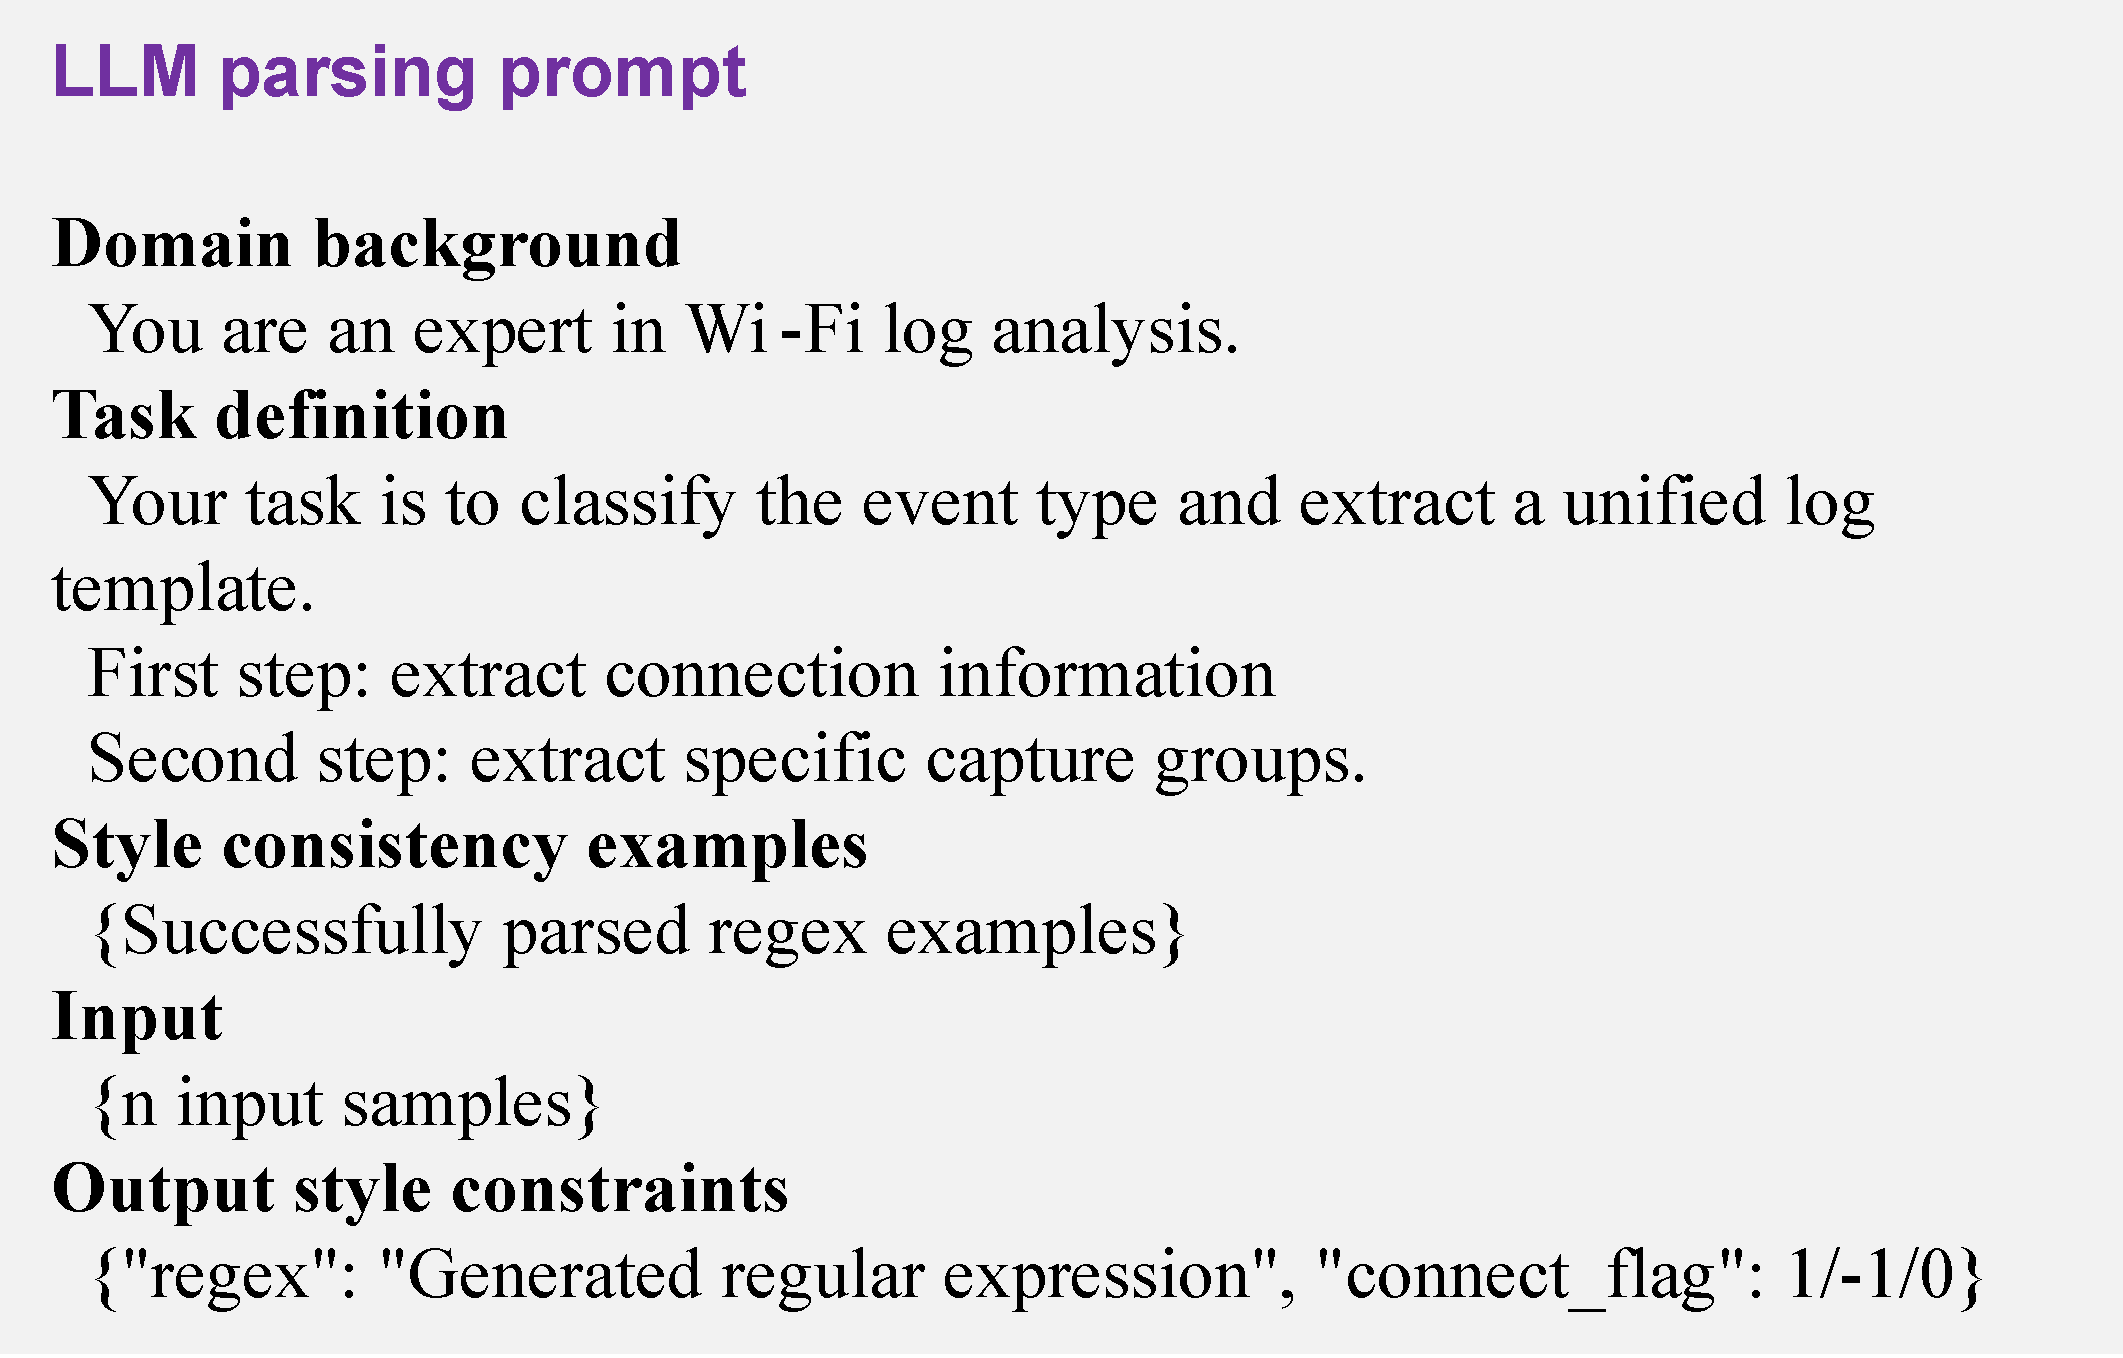
\includegraphics[width=0.95\linewidth]{figure/Picture6.pdf}}\\[0.6ex]
	\subfloat[Regex self-repair prompt structure]{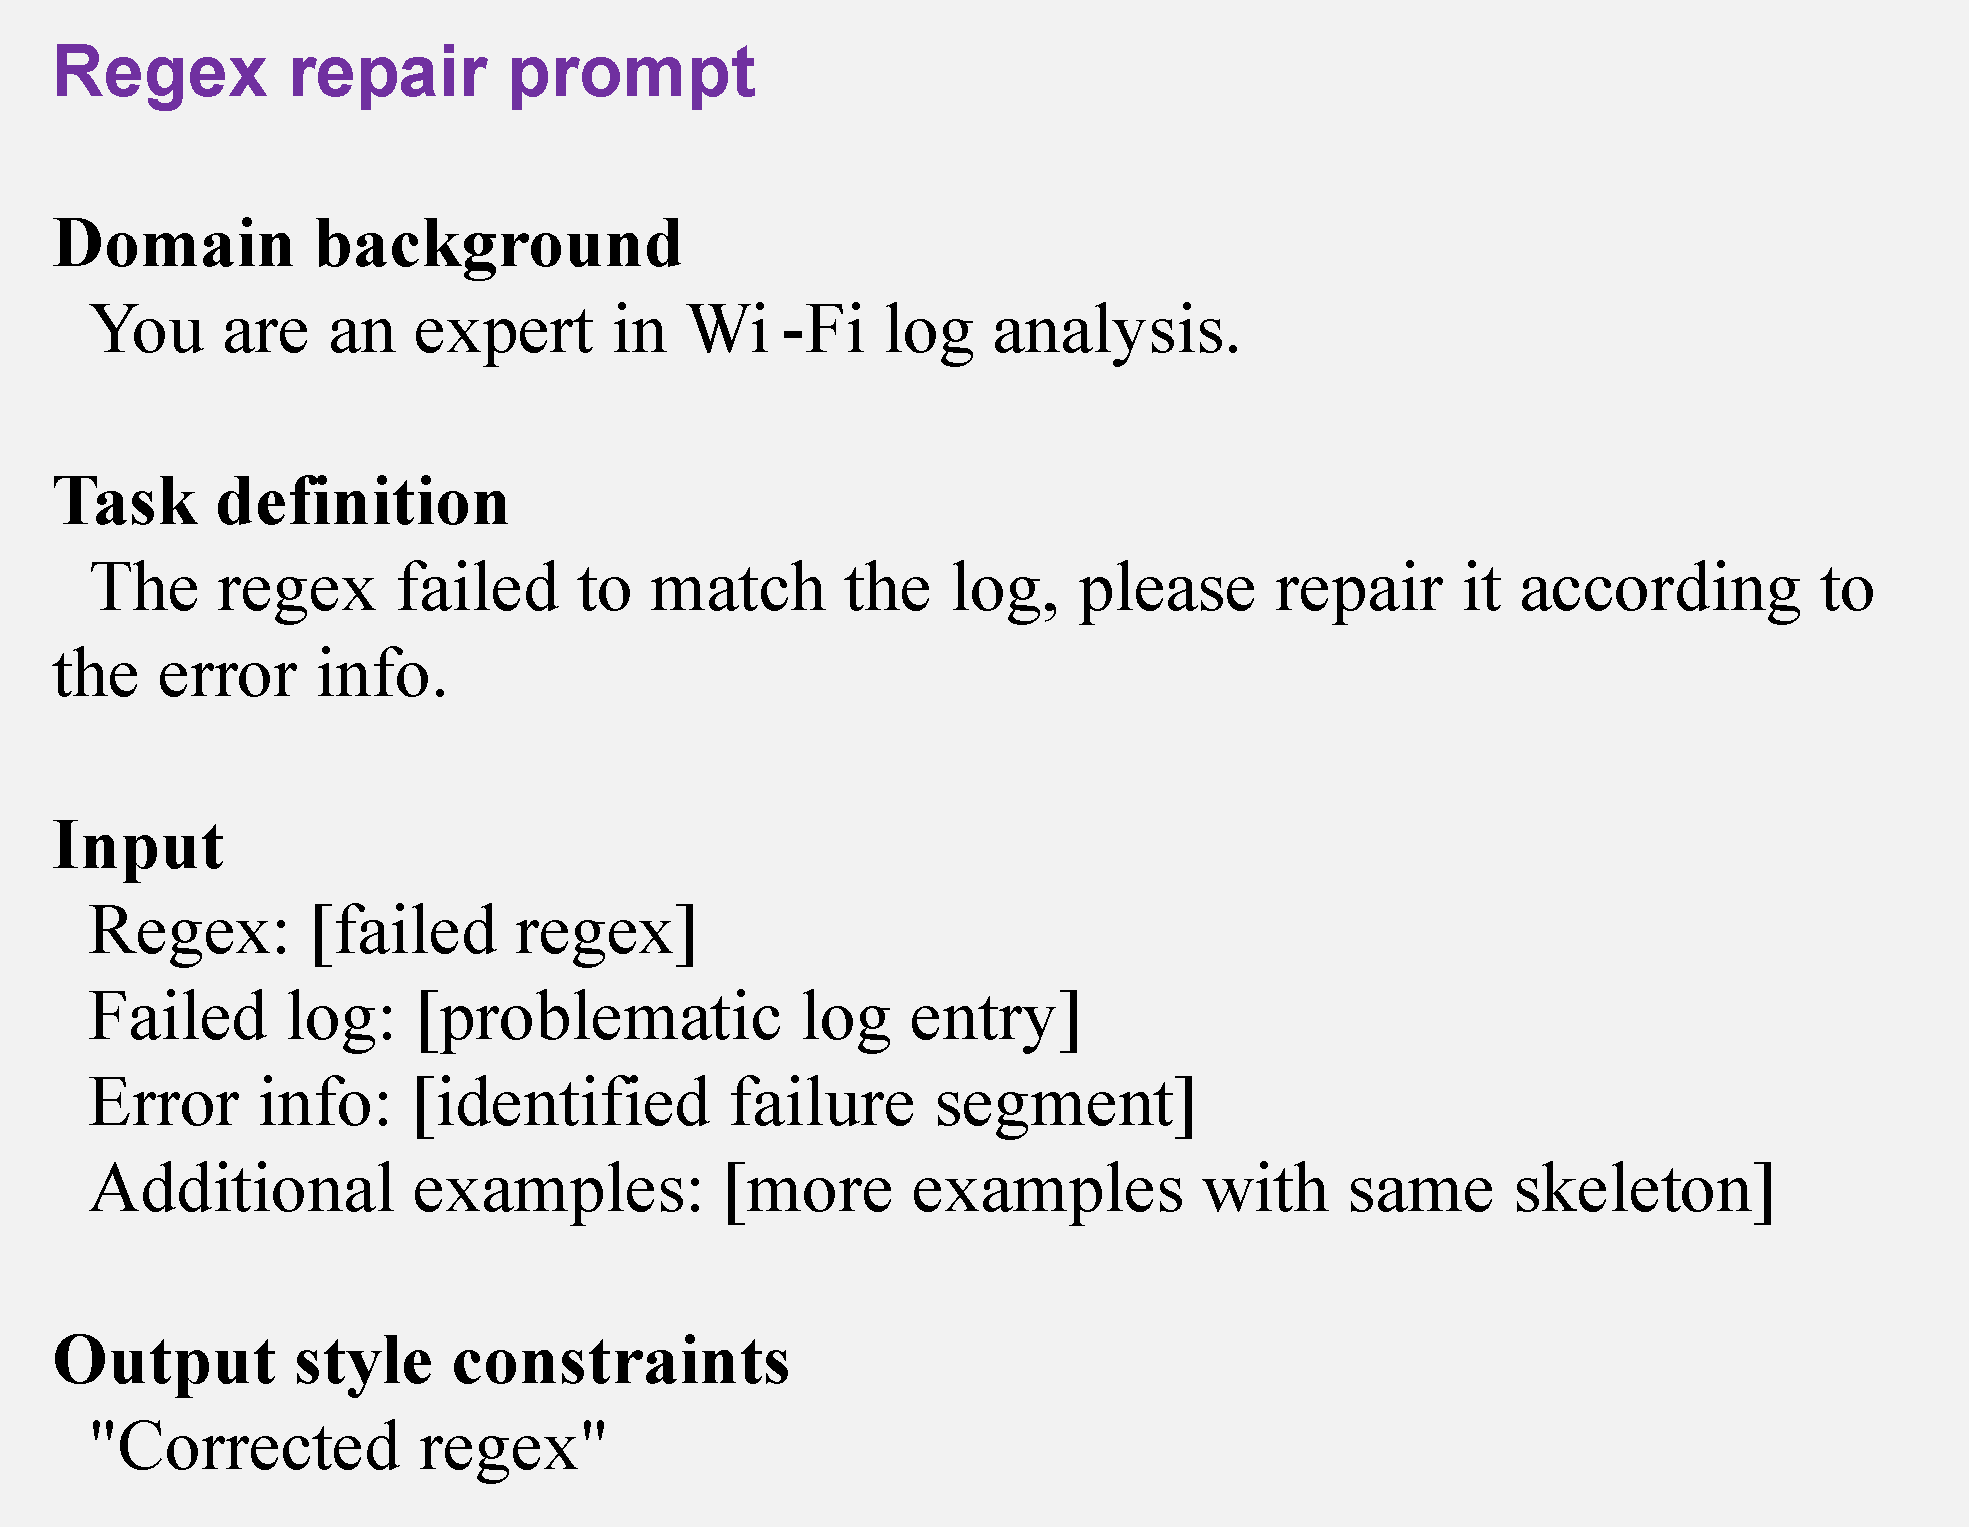
\includegraphics[width=0.95\linewidth]{figure/Picture7.pdf}}
	\caption{Prompt structure sketches used for (a) timestamp header induction, (b) micro-group parser induction, and (c) bounded self-repair.}
	\label{fig:prompt_sketch}
\end{figure}

\subsection{Overall Parsing Flow and Parser Cache}
Algorithm~\ref{alg:main} summarizes the end-to-end parsing flow across Steps~1--4. WiFiLogParser maintains a parser library that stores validated parsers, together with a structural signature index that maps structural signatures to parser IDs. With consolidation, multiple micro-groups can share the same parser.

\begin{algorithm}[!t]
	\caption{WiFiLogParser (overview).}
	\label{alg:main}
	\begin{algorithmic}[1]
		\STATE \textbf{Input:} log lines $\mathcal{L}$
		\STATE \textbf{Output:} mobility records $\mathcal{R}$
		\STATE $H \leftarrow \textsc{InduceHeader}(\mathcal{L})$ \COMMENT{Appendix~A}
		\STATE $(\mathcal{T},\mathcal{C}) \leftarrow \textsc{SplitHeaderContent}(\mathcal{L}, H)$ \COMMENT{timestamps, contents}
		\STATE $\mathcal{G} \leftarrow \textsc{GroupBySignature}(\mathcal{C})$ \COMMENT{micro-groups}
		\STATE initialize parser library $\mathcal{P}$
		\FORALL{micro-group $g \in \mathcal{G}$}
		\STATE $p \leftarrow \textsc{LookupParser}(\mathcal{P}, g)$
		\IF{$p = \emptyset$}
		\STATE $\mathcal{S} \leftarrow \textsc{SampleRepresentatives}(g)$
		\STATE $p \leftarrow \textsc{InduceParserWithLLM}(\mathcal{S})$ \COMMENT{regex + label}
		\STATE $p \leftarrow \textsc{ValidateAndRepair}(p, g)$ \COMMENT{Appendix~B}
		\STATE $\mathcal{P} \leftarrow \mathcal{P} \cup \{p\}$
		\STATE \textsc{ConsolidateParsers}($\mathcal{P}$, $\mathcal{G}$, $p$) \COMMENT{merge covered groups}
		\ENDIF
		\STATE $\mathcal{R} \leftarrow \mathcal{R} \cup \textsc{ParseGroup}(p, g, \mathcal{T})$
		\ENDFOR
		\STATE \textbf{return} $\mathcal{R}$
	\end{algorithmic}
\end{algorithm}

WiFiLogParser stores each validated parser as a reusable library entry, including its structural signature(s), the regex, and the event label. This cache is the main driver of scalability: once a parser is learned for a recurring log structure, subsequent occurrences are handled by deterministic regex matching without additional LLM calls. A conceptual example of the parser cache entry and many-to-one micro-group-to-parser sharing is shown in Fig.~\ref{fig:cache}.


\begin{figure}[!t]

	\centering
	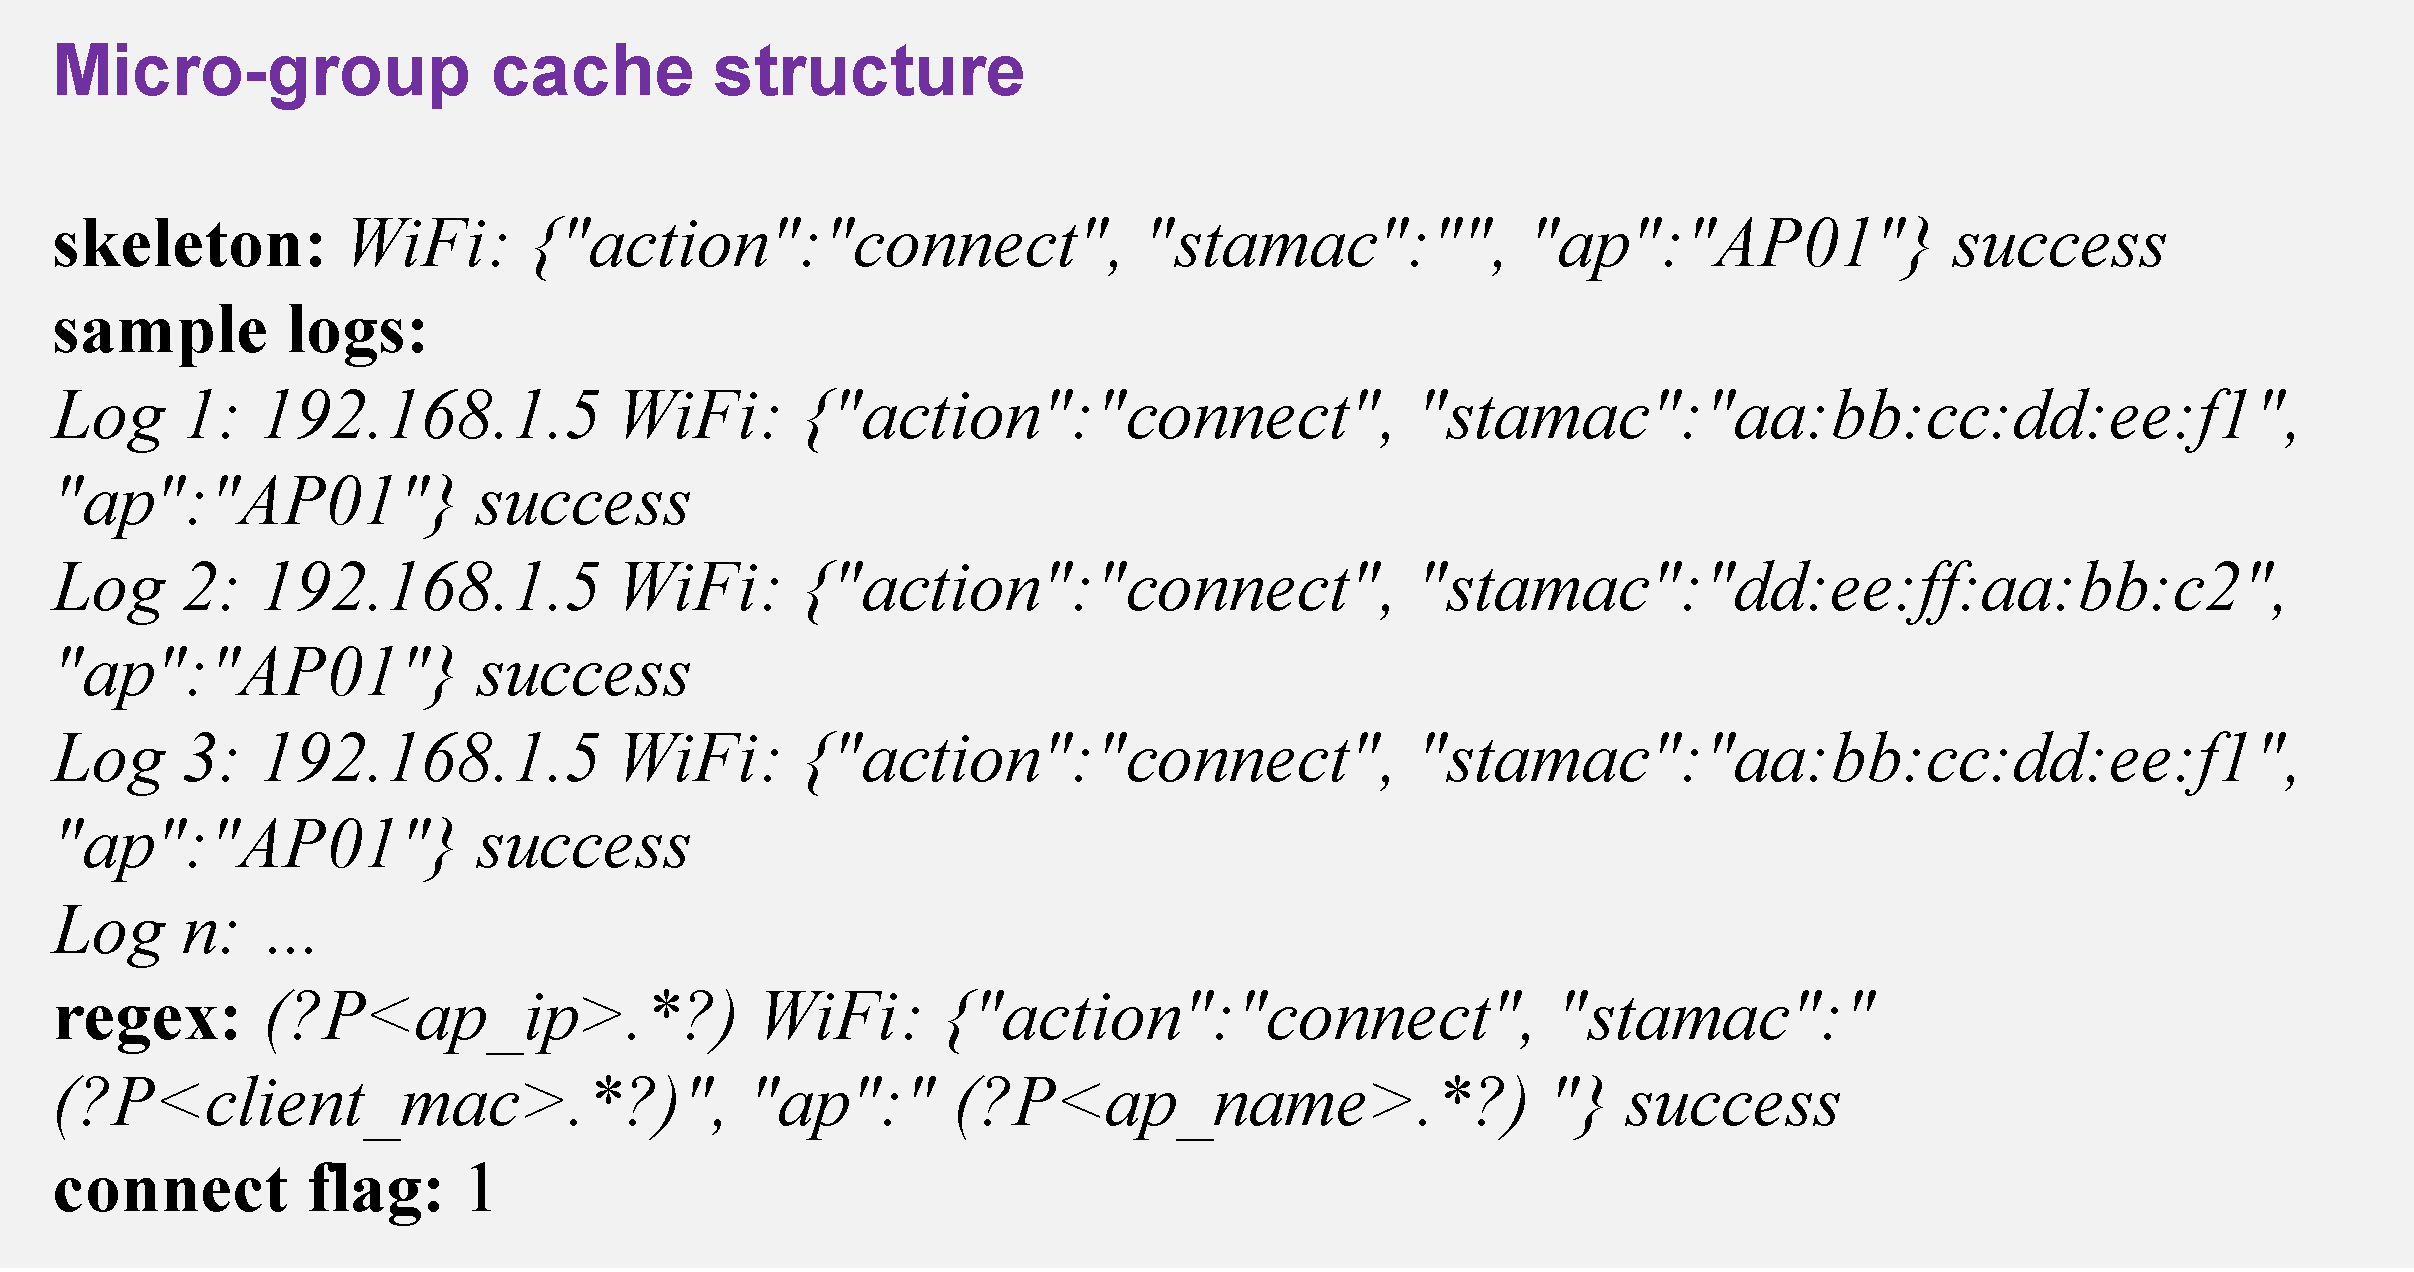
\includegraphics[width=\linewidth]{figure/Picture4.pdf}
	\caption{Conceptual cache entry for a micro-group. Consolidation allows multiple micro-groups to share one parser entry.}
	\label{fig:cache}
\end{figure}

\section{Experimental Setup}
\subsection{Datasets}


We evaluate WiFiLogParser on three real-world Wi-Fi log datasets from different vendors (Table~\ref{tab:datasets}). The University dataset (Aruba) uses syslog-style messages and includes embedded structured payloads in some event traces. The Wilson dataset (Ubiquiti) contains key-value style event logs with frequent embedded JSON segments. The Holly Springs (HS) dataset (Fortinet) is provided in a CSV-like export format. Representative raw-log examples from the University, Wilson, and HS datasets are shown in Fig.~\ref{fig:examples}.


\begin{table*}[!t]
	\centering
	\caption{Description of Wi-Fi log datasets.}
	\label{tab:datasets}
	\begin{tabular}{cccccc}
		\toprule
		\textbf{Location}         & \textbf{Wi-Fi Provider} & \textbf{Area} & \textbf{\#APs} & \textbf{Data Size}       & \textbf{Period}                  \\
		\midrule
		UNC Charlotte             & HPE Aruba               & 1.56 mi$^2$   & 2,492          & 380 MB (2,074,634 lines) & 00:25--23:59 1/1/2021            \\
		City of Wilson, NC        & Ubiquiti                & 23 mi$^2$     & 292            & 316 MB (1,496,693 lines) & 14:48--19:10 2/14/2024           \\
		Town of Holly Springs, NC & Fortinet                & 15 mi$^2$     & 55             & 6 MB (36,449 lines)      & 00:00 7/16/2023--17:17 7/17/2023 \\
		\bottomrule
	\end{tabular}
\end{table*}


\begin{figure*}[!t]

	\centering
	\subfloat[University]{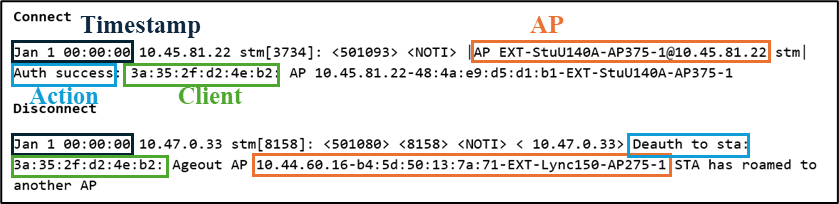
\includegraphics[width=0.7\linewidth]{figure/Picture8a.png}}\\
	\vspace{-0.3cm}
	\subfloat[Wilson]{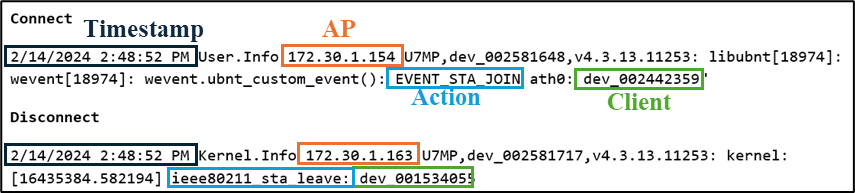
\includegraphics[width=0.7\linewidth]{figure/Picture8b.png}}\\
	\vspace{-0.3cm}
	\subfloat[HS]{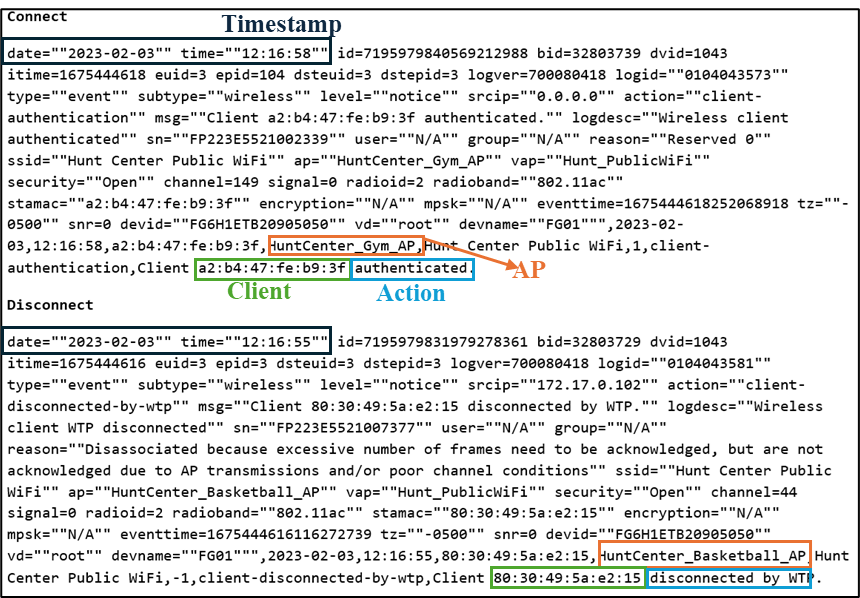
\includegraphics[width=0.7\linewidth]{figure/Picture8c.png}}
	\caption{Example Wi-Fi logs from the three datasets.}
	\label{fig:examples}
\end{figure*}

\textbf{Ground truth annotation.} For each dataset, we inspect log semantics and vendor conventions and implement a dataset-specific annotation script that assigns each line $y\in\{1,-1,0\}$ following IEEE 802.11 association/authentication vs. disassociation/deauthentication state transitions \cite{ref55}. These scripts are used only to generate evaluation labels and are not used by WiFiLogParser or the compared baselines.


\subsection{Evaluation Metrics}

\textbf{Event classification.}
We evaluate event type prediction over three classes
$C=\{1,-1,0\}$, corresponding to connection, disconnection,
and no event, respectively.
For each class $c\in C$, we adopt a one-vs-rest scheme and define

\begin{align}
	\mathrm{TP}_c & = \sum_{i=1}^{n} \mathbf{1}\{y_i=c \land \hat{y}_i=c\}, \nonumber     \\
	\mathrm{FP}_c & = \sum_{i=1}^{n} \mathbf{1}\{y_i\neq c \land \hat{y}_i=c\}, \nonumber \\
	\mathrm{FN}_c & = \sum_{i=1}^{n} \mathbf{1}\{y_i=c \land \hat{y}_i\neq c\},
\end{align}

where TP/FP/FN denote true positives/false positives/false negatives, $\hat{y}_i$ denotes the predicted label for line $i$, and
$\mathbf{1}\{\cdot\}$ is the indicator function.

For each class $c$, precision, recall, and F1 score are defined as

\begin{align}
	\mathrm{Precision}_c & =
	\frac{\mathrm{TP}_c}{\mathrm{TP}_c+\mathrm{FP}_c}, \nonumber \\
	\mathrm{Recall}_c    & =
	\frac{\mathrm{TP}_c}{\mathrm{TP}_c+\mathrm{FN}_c}, \nonumber \\
	\mathrm{F1}_c        & =
	\frac{2\,\mathrm{Precision}_c\,\mathrm{Recall}_c}
	{\mathrm{Precision}_c+\mathrm{Recall}_c}.
\end{align}

The event classification metric is the overall F1 as the macro-average over the three classes:

\begin{align}
	\mathrm{F1}
	=
	\frac{1}{|C|}
	\sum_{c\in C}
	\mathrm{F1}_c.
\end{align}


\textbf{Field extraction accuracy (FEA).} For lines labeled as connection/disconnection events in the ground truth, we measure the per-field extraction accuracy for the six non-temporal fields (AP/client name, IP, and MAC) and average across $k=6$ fields:
\begin{align}
	A_f        & = \frac{c_f}{n_m}, \nonumber     \\
	\text{FEA} & = \frac{1}{k}\sum_{f=1}^{k} A_f,
\end{align}
where $c_f$ counts the number of event lines whose field $f$ is extracted exactly (including correctly predicting an empty value), and $n_m$ is the number of event lines in the ground truth. The timestamp is extracted by Step~1 and is not included in FEA.

\textbf{Efficiency.} We report LLM API call counts, token usage, and time spent in LLM parsing operations (including I/O and preprocessing), following common practice in log parsing system evaluations.

\subsection{Baselines and Implementation Settings}
To contextualize WiFiLogParser, we compare it against two categories of baselines.

\textbf{Direct LLM.} We prompt an LLM to parse raw log lines directly into structured mobility records. Due to the high token cost of per-line parsing, we evaluate Direct LLM on a 2,000-line subset per dataset. Each LLM call processes 40 lines and returns CSV rows, which are concatenated to form the final output.

\textbf{Template parsing + post-processing (LILAC$+$ / LogBatcher$+$).} LLM-based parsers such as LILAC \cite{ref30} and LogBatcher \cite{ref32} mainly output templates. To make this output comparable to our mobility schema, we follow the natural ``template then semantic labeling'' workflow and add two rounds of LLM post-processing. First, we label each induced template with an event type $y\in\{1,-1,0\}$. Second, for templates predicted as connection/disconnection ($y\neq 0$), we prompt the same LLM to generate a full-line regex with named capture groups that extracts our AP/client fields. We then propagate the template label and regex to all raw lines mapped to that template and compute F1/FEA. We denote these aligned pipelines as LILAC$+$ and LogBatcher$+$.

\textbf{Ablation.} We conduct two ablations: (i) with vs. without Self-Repair, and (ii) replacing structural-signature micro-grouping with unsupervised clustering from LogBatcher while keeping the remaining pipeline unchanged.

\textbf{Fairness and configuration.} Unless otherwise specified, all LLM calls use the same backend (Gemini-2.0-Flash \cite{ref38}) with temperature 0. To ensure a fair comparison for mobility extraction, we apply the same timestamp-header filtering rule to all methods and evaluate only on lines with detectable timestamps.

\section{Results and Analysis}
\label{sec:results}


\subsection{Experiment 1: Small-scale Evaluation and Results}
\label{subsec:direct_llm_subset}
Per-line LLM parsing is an informative but costly reference point. We therefore evaluate Direct LLM on a 2,000-line subset per dataset and report the results in Table~\ref{tab:subset_2000}. All methods in this table are evaluated on the same 2,000-line subsets to keep the comparison controlled.

\begin{table}[!t]
	\centering
	\caption{Performance on 2,000-line subsets.}
	\label{tab:subset_2000}
	\footnotesize
	\setlength{\tabcolsep}{4pt}
	\begin{tabular}{lcccccc}
		\toprule
		\multirow{2}{*}{\textbf{Method}}        &
		\multicolumn{2}{c}{\textbf{Wilson}}     &
		\multicolumn{2}{c}{\textbf{University}} &
		\multicolumn{2}{c}{\textbf{HS}}                                                                                                         \\
		\cmidrule(lr){2-3}\cmidrule(lr){4-5}\cmidrule(lr){6-7}
		                                        & \textbf{F1}   & \textbf{FEA}  & \textbf{F1}   & \textbf{FEA}  & \textbf{F1}   & \textbf{FEA}  \\
		\midrule
		Direct LLM                              & 0.94          & 0.88          & 0.82          & 0.90          & 0.97          & 0.99          \\
		LILAC$+$                                & 0.69          & 0.70          & 0.75          & 0.73          & 0.72          & 0.85          \\
		LogBatcher$+$                           & 0.73          & 0.68          & 0.76          & 0.75          & 0.69          & 0.89          \\
		WiFiLogParser                           & \textbf{0.99} & \textbf{0.97} & \textbf{0.84} & \textbf{0.92} & \textbf{0.97} & \textbf{1.00} \\
		\bottomrule
	\end{tabular}
\end{table}

Table~\ref{tab:subset_2000} shows that WiFiLogParser achieves the best accuracy on all three 2,000-line subsets, with the largest gains over the template-centered baselines. On Wilson, WiFiLogParser improves from baseline-best F1=0.73 (LogBatcher$+$) and baseline-best FEA=0.70 (LILAC$+$) to 0.99/0.97. On University, it improves from 0.76/0.75 (LogBatcher$+$) to 0.84/0.92. On HS, it improves from 0.72/0.89 (LILAC$+$/LogBatcher$+$) to 0.97/1.00. Relative to Direct LLM, WiFiLogParser delivers comparable or better accuracy (e.g., Wilson: 0.94/0.88 $\rightarrow$ 0.99/0.97) while avoiding per-line parsing. The pattern is that micro-group parser induction preserves small-scale accuracy while substantially improving role-aware field extraction over template outputs.

\subsection{Experiment 2: Full Datasets Evaluation and Results}
\label{subsec:main_perf}

Table~\ref{tab:main_full} shows that WiFiLogParser maintains strong end-to-end accuracy on the full datasets, achieving F1/FEA of 0.999/0.998 (Wilson), 0.916/0.924 (University), and 0.994/1.000 (HS). Compared with LogBatcher$+$, WiFiLogParser improves event F1 by 23.9/12.6/31.4 percentage points and FEA by 21.8/16.4/15.0 percentage points on Wilson/University/HS, respectively. The persistent gap suggests a limitation of template-level post-processing in this mobility-extraction setting: templates abstract away role semantics, and propagating template-level labels/regex to all mapped lines can amplify errors. These results indicate that WiFiLogParser can scale to million-scale heterogeneous logs while preserving high event and field extraction quality.


\begin{table}[!t]
	\centering
	\caption{End-to-end performance on full datasets.}
	\label{tab:main_full}
	\footnotesize
	\setlength{\tabcolsep}{4pt}
	\begin{tabular}{lcccccc}
		\toprule
		\multirow{2}{*}{\textbf{Method}}        &
		\multicolumn{2}{c}{\textbf{Wilson}}     &
		\multicolumn{2}{c}{\textbf{University}} &
		\multicolumn{2}{c}{\textbf{HS}}                                                                                                               \\
		\cmidrule(lr){2-3}\cmidrule(lr){4-5}\cmidrule(lr){6-7}
		                                        & \textbf{F1}    & \textbf{FEA}   & \textbf{F1}    & \textbf{FEA}   & \textbf{F1}    & \textbf{FEA}   \\
		\midrule
		LILAC$+$                                & 0.720          & 0.740          & 0.700          & 0.740          & 0.690          & 0.830          \\
		LogBatcher$+$                           & 0.760          & 0.780          & 0.790          & 0.760          & 0.680          & 0.850          \\
		WiFiLogParser                           & \textbf{0.999} & \textbf{0.998} & \textbf{0.916} & \textbf{0.924} & \textbf{0.994} & \textbf{1.000} \\
		\bottomrule
	\end{tabular}
\end{table}


\subsection{Efficiency and Cost}
\label{subsec:efficiency}
Table~\ref{tab:efficiency} compares the LLM call count, token usage, and time spent on the full datasets. For comparability across datasets, we report the average cost per 1,000 lines.

For Direct LLM, each call parses a batch of 40 lines and we evaluate on a 2,000-line subset per dataset (50 calls total); we then normalize calls/tokens/time to ``per 1,000 lines'' (thus 25 calls per 1,000 lines).

\begin{table*}[!t]
	\centering
	\caption{Efficiency comparison per 1,000 lines. Direct LLM values are normalized from 2,000-line runs with 40 lines per call.}
	\label{tab:efficiency}
	\begin{tabular}{lccc|ccc|ccc}
		\toprule
		\multirow{2}{*}{\textbf{Method}}         &
		\multicolumn{3}{c|}{\textbf{Wilson}}     &
		\multicolumn{3}{c|}{\textbf{University}} &
		\multicolumn{3}{c}{\textbf{HS}}                                                                                                                                                                 \\
		\cmidrule(lr){2-4}\cmidrule(lr){5-7}\cmidrule(lr){8-10}
		                                         & \textbf{calls}   & \textbf{time(s)} & \textbf{tokens}  &
		\textbf{calls}                           & \textbf{time(s)} & \textbf{tokens}  &
		\textbf{calls}                           & \textbf{time(s)} & \textbf{tokens}                                                                                                                   \\
		\midrule
		Direct LLM                               & 25               & 56               & 133{,}124        & 25           & 72           & 110{,}242    & 25           & 74           & 187{,}261        \\
		LILAC$+$                                 & 0.8              & 0.9              & 2{,}158          & 1.5          & 2.7          & 2{,}268      & 1.1          & 2.1          & 3{,}182          \\
		LogBatcher$+$                            & 0.7              & 0.8              & 1{,}442          & 1.2          & 2.3          & 1{,}974      & 1.3          & 2.3          & 2{,}513          \\
		\midrule
		WiFiLogParser                            & \textbf{0.5}     & \textbf{0.7}     & \textbf{1{,}037} & \textbf{0.2} & \textbf{0.2} & \textbf{310} & \textbf{1.1} & \textbf{1.9} & \textbf{1{,}040} \\
		\bottomrule
	\end{tabular}
\end{table*}

Table~\ref{tab:efficiency} confirms that Direct LLM is not scalable under per-line cost: it requires 25 calls and 110k--187k tokens per 1,000 lines. WiFiLogParser reduces the overhead to 0.5/0.2/1.1 calls, 0.7/0.2/1.9 seconds, and 1{,}037/310/1{,}040 tokens per 1,000 lines on Wilson/University/HS. Even relative to the aligned template pipelines, WiFiLogParser uses fewer tokens because it jointly induces an event label and a regex per micro-group and then reuses cached parsers; most lines are processed deterministically after cache hits. Overall, WiFiLogParser achieves near-direct accuracy on subsets while reducing LLM calls, tokens, and time by orders of magnitude at scale.

\subsection{Ablation Studies}
\label{subsec:ablation}

\subsubsection{Ablation 1: Failure Localization and Self-Repair}
We evaluate WiFiLogParser with and without the self-repair mechanism. With our default backend (Gemini-2.0-Flash), self-repair improves field extraction on Wilson (FEA: 0.99 $\rightarrow$ 1.00) and University (0.91 $\rightarrow$ 0.93), while HS remains saturated (1.00 in both settings), as shown in Table~\ref{tab:ablation_repair}.

\begin{table}[!t]
	\centering
	\caption{Ablation of self-repair (Gemini-2.0-Flash): FEA on event logs with vs. without self-repair.}
	\label{tab:ablation_repair}
	\begin{tabular}{lcc}
		\toprule
		\textbf{Dataset} & \textbf{w/o self-repair} & \textbf{w/ self-repair} \\
		\midrule
		Wilson           & 0.99                     & \textbf{1.00}           \\
		University       & 0.91                     & \textbf{0.93}           \\
		HS               & 1.00                     & 1.00                    \\
		\bottomrule
	\end{tabular}
\end{table}

\subsubsection{Ablation 2: Structural Signatures and Greedy Consolidation vs. Unsupervised Clustering}


Structural signatures can fragment when entity values (e.g., SSIDs and AP names) or embedded structured payloads vary. Consolidation directly targets this issue by merging micro-groups under a shared validated parser, thereby reducing the number of distinct parsers. As shown in Table~\ref{tab:consolidation}, HS reduces from 993 micro-groups to 32 consolidated parser buckets, University reduces from 646 to 187, and Wilson reduces from 474 to 330.



\begin{table}[!t]
	\centering
	\caption{Effect of coverage-driven consolidation on signature fragmentation.}
	\label{tab:consolidation}
	\begin{tabular}{lcc}
		\toprule
		\textbf{Dataset} & \textbf{Micro-groups} & \textbf{Parser buckets} \\
		\midrule
		University       & 646                   & 187                     \\
		Wilson           & 474                   & 330                     \\
		HS               & 993                   & 32                      \\
		\bottomrule
	\end{tabular}
\end{table}

Consolidation reduces the number of parser inductions because one validated parser is shared across all signatures in the same bucket. The reduction is substantial for HS (993 $\rightarrow$ 32, 96.8\%) and University (646 $\rightarrow$ 187, 71.1\%), indicating that many structural signatures are fragmented by high-entropy tokens rather than truly different structures. Wilson shows a smaller reduction (474 $\rightarrow$ 330, 30.4\%), suggesting more genuinely distinct message forms and embedded payload variation. This ``split first for purity, then merge by coverage'' strategy increases parser reuse and controls LLM cost.

To quantify how much semantic purity depends on pre-grouping, we replace structural signature micro-grouping with unsupervised clustering from LogBatcher while keeping the rest of the pipeline unchanged. Table~\ref{tab:ablation_grouping} shows that the main degradation is in event classification (Avg. F1: 0.96 vs. 0.77), while field extraction accuracy remains similar (Avg. FEA: 0.97 vs. 0.96).

\begin{table}[!t]
	\centering
	\caption{Ablation of pre-grouping strategy (average over datasets).}
	\label{tab:ablation_grouping}
	\begin{tabular}{lcc}
		\toprule
		\textbf{Pre-grouping}                     & \textbf{Avg. F1} & \textbf{Avg. FEA} \\
		\midrule
		Unsupervised clustering (from LogBatcher) & 0.77             & 0.96              \\
		Split-for-purity + consolidation (ours)   & \textbf{0.96}    & \textbf{0.97}     \\
		\bottomrule
	\end{tabular}
\end{table}

Empirically, unsupervised clustering often merges distinct Wi-Fi events into one cluster; in our setting, this is associated with lower event F1 (Table~\ref{tab:ablation_grouping}). A plausible reason is that assigning one label to a mixed cluster biases predictions toward the dominant non-event pattern, increasing false negatives for connection events.

\section{Case Study: From Logs to Mobility Flows}
To make downstream utility concrete, we link extracted mobility events to AP locations and visualize aggregated flows. For the University deployment, the extracted mobility records cover thousands of client devices and dozens of APs with known coordinates. We construct AP-to-AP transition counts from consecutive client connections and plot the most frequent transitions over AP coordinates. Fig.~\ref{fig:case_flow} shows the visualization of the AP hotspots and flow within the university Wi-Fi coverage area, which provides unique insights into movement patterns on campus.

\begin{figure}[!t]
	\centering
	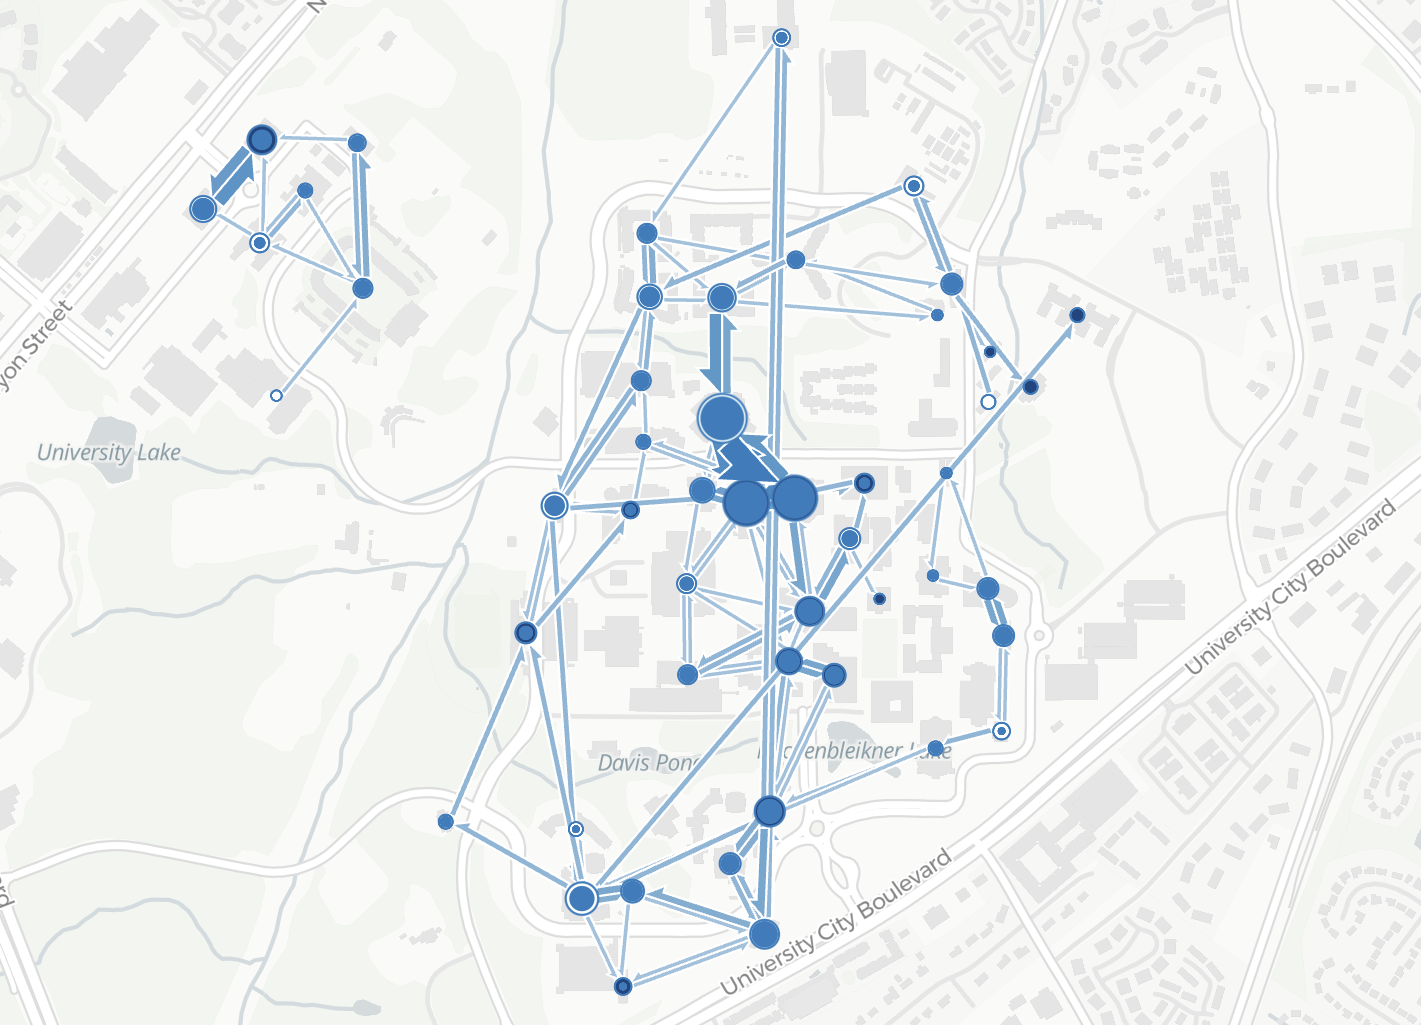
\includegraphics[width=\linewidth]{figure/Picture_case_university.png}
	\caption{Case study visualization (University). Points show AP locations sized by observed connection events; lines show the most frequent AP-to-AP transitions inferred from consecutive client connections.}
	\label{fig:case_flow}
\end{figure}


\section{Conclusion}
WiFiLogParser provides an end-to-end LLM-based approach for extracting Wi-Fi mobility records from heterogeneous raw logs. It automatically induces timestamp header patterns, performs semantic parsing by inducing reusable parsers (named-group regex paired with event labels), and consolidates fragmented micro-groups through regex coverage validation and caching. On complete datasets, WiFiLogParser achieves F1-scores of 0.916--0.999 and FEA of 0.924--1.000; relative to a Direct LLM baseline, it reduces token consumption by over 99\% and cuts LLM calls and LLM-only runtime by 98\%+ in per-1,000-line cost estimates.

\textbf{Limitations and future work.} WiFiLogParser is designed for Wi-Fi mobility extraction and may require schema adaptation for other system logs. This is particularly true for the structural signature rules, which are a task-specific heuristic approach. How to semantically parse and analyze various system logs remains an open problem. Future work can explore extending WiFiLogParser to other log types and schemas.

\appendices
\section{Coverage-driven Timestamp Header Parsing}
\label{app:header}
Algorithm~\ref{alg:header} sketches the coverage-driven procedure used by \textsc{InduceHeader} (Step~1). Across refinements and restarts, we keep track of the regex with the best match coverage.

\begin{algorithm}[!t]
	\caption{\textsc{InduceHeader} (sketch).}
	\label{alg:header}
	\begin{algorithmic}[1]
		\STATE \textbf{Input:} raw lines $\{l_i\}$
		\STATE \textbf{Params:} $n{=}10$, $\Delta{=}3$, $\tau{=}0.95$, maxRefineRounds$=10$, restart\_max$=3$
		\STATE $bestH \leftarrow \emptyset$, $bestCov \leftarrow 0$
		\FOR{restart $=1$ to restart\_max}
		\STATE $\mathcal{S} \leftarrow$ select $n$ diverse samples from $\{l_i\}$
		\STATE $H \leftarrow$ LLM-proposed header regex from $\mathcal{S}$
		\FOR{round $=1$ to maxRefineRounds}
		\STATE $\mathcal{U} \leftarrow \{l_i : H \text{ does not match } l_i\}$
		\STATE $cov \leftarrow 1 - |\mathcal{U}|/|\{l_i\}|$
		\IF{$cov > bestCov$} \STATE $bestCov \leftarrow cov$; $bestH \leftarrow H$ \ENDIF
		\IF{$cov \ge \tau$} \STATE \textbf{return} $H$ \ENDIF
		\STATE $\Delta\mathcal{S} \leftarrow$ select $\Delta$ diverse samples from $\mathcal{U}$
		\STATE $H \leftarrow$ LLM refine $H$ given $\mathcal{S} \cup \Delta\mathcal{S}$
		\STATE $\mathcal{S} \leftarrow \mathcal{S} \cup \Delta\mathcal{S}$
		\ENDFOR
		\ENDFOR
		\STATE \textbf{return} $bestH$ \COMMENT{Best-effort header}
	\end{algorithmic}
\end{algorithm}

\section{Regex Validation and Self-Repair}
\label{app:repair}
Algorithm~\ref{alg:repair} sketches the bounded \textsc{ValidateAndRepair} procedure (Step~4). All LLM repair attempts are counted as LLM calls in Table~\ref{tab:efficiency}.

\begin{algorithm}[!t]
	\caption{\textsc{ValidateAndRepair} (sketch).}
	\label{alg:repair}
	\begin{algorithmic}[1]
		\STATE \textbf{Input:} parser $p$ (regex + label), group $g$
		\STATE \textbf{Params:} repair budget $T$
		\FOR{$t=1$ to $T$}
		\IF{\textsc{Valid}$(p,g)$} \STATE \textbf{return} $p$ \ENDIF
		\STATE info $\leftarrow$ \textsc{DiagnoseMismatch}$(p,g)$
		\STATE $p \leftarrow$ \textsc{RepairWithLLM}$(p,\text{info})$
		\ENDFOR
		\STATE \textbf{return} \textsc{Fail}
	\end{algorithmic}
\end{algorithm}

\bibliographystyle{IEEEtran}
\bibliography{references}

\end{document}
